\documentclass[a4paper, 12pt, twoside]{book}

%%%%%%%%%%%%%%%%%%%%%%%%%%%%%%%%%%%%%%%%%%%%%%%%%%%%%%%%%%%%%%%%%%%%%%%%%%%%%%%%%%%%%%%%%%%%%%%%%%%%%%%%%%% paketi
\usepackage[utf8x]{inputenc} % omogoča uporabo slovenskih črk kodiranih v formatu UTF-8 
\usepackage[slovene,english]{babel} % naloži, med drugim, slovenske delilne vzorce
\usepackage[pdftex]{graphicx} % omogoča vlaganje slik različnih formatov 
\usepackage[tmargin=3cm,rmargin=2cm,bmargin=3cm,lmargin=3cm]{geometry} % nastavi pravilne odmike
\usepackage{listings} % izvorna koda
\usepackage{pxfonts} % omogoča krepko pisavo v izvorni kodi
\usepackage[hyphens]{url} % url naslovi v virih

%%%%%%%%%%%%%%%%%%%%%%%%%%%%%%%%%%%%%%%%%%%%%%%%%%%%%%%%%%%%%%%%%%%%%%%%%%%%%%%%%%%%%%%%%%%%%%%%%%%%%%% nastavitve
\renewcommand{\baselinestretch}{1.3} % ustrezen razmik med vrsticami
% \setcounter{tocdepth}{1} % globina kazala
\newcommand{\clearemptydoublepage}{\newpage{\pagestyle{empty}\cleardoublepage}} % prazne strani

%%%%%%%%%%%%%%%%%%%%%%%%%%%%%%%%%%%%%%%%%%%%%%%%%%%%%%%%%%%%%%%%%%%%%%%%%%%%%%%%%%%%%%%%%%%%%%%%%%%%% izvorna koda
\lstset{
	basicstyle=\footnotesize\ttfamily, % pomanjšana pisava in monospace
	breaklines=true, % prelom vrstic
	captionpos=b, % napis na dnu
	frame=top, % črta zgoraj
	frame=bottom, % črta spodaj
	keywordstyle=\bfseries, % krepka pisava
	morekeywords={function, var, this, self}, % poudarjene besede
	numbers=left, % oznaka vrstice
	numberstyle=\tiny, % majcena pisava za oznake vrstic
	tabsize=2, % dva presledka zamika kode
	escapeinside={@}{@}, % koda znotraj afne se ignorira
	title=\lstname
}

%%%%%%%%%%%%%%%%%%%%%%%%%%%%%%%%%%%%%%%%%%%%%%%%%%%%%%%%%%%%%%%%%%%%%%%%%%%%%%%%%%%%%%%%%%%%%%%%%%%%%%%%%%%%%%%%%%
\begin{document}
\selectlanguage{slovene}

%%%%%%%%%%%%%%%%%%%%%%%%%%%%%%%%%%%%%%%%%%%%%%%%%%%%%%%%%%%%%%%%%%%%%%%%%%%%%%%%%%%%%%%%%%%%%%%%%%% naslovna stran
\thispagestyle{empty}
\begin{center}
	{\large\sc Univerza v Ljubljani \par}
	{\large\sc Fakulteta za računalništvo in informatiko \par}
	\vskip 14em
	{\Large Marko Bregant \par}
	\vskip 1em
	{\huge\bf Operativna transformacija \par}
	\vskip 2em
	{\normalsize\sc DIPLOMSKO DELO \par }
	\vskip 0.8em
	{\normalsize\sc UNIVERZITETNI ŠTUDIJSKI PROGRAM PRVE STOPNJE \par }
	{\normalsize\sc RAČUNALNIŠTVO IN INFORMATIKA \par }
	\vfill
	{\large \textsc{Mentor}: doc. dr. Zoran Bosnić \par}
	\vskip 2em
	{\large Ljubljana 2014 \par}
\end{center}

\clearemptydoublepage

%%%%%%%%%%%%%%%%%%%%%%%%%%%%%%%%%%%%%%%%%%%%%%%%%%%%%%%%%%%%%%%%%%%%%%%%%%%%%%%%%% izjava o intelektualni lastnini
\thispagestyle{empty}
\vspace*{11cm}
{\small \noindent Rezultati diplomskega dela so intelektualna lastnina avtorja in Fakultete za ra\-ču\-nal\-niš\-tvo in informatiko Univerze v Ljubljani. Za objavljanje ali izkoriščanje rezultatov di\-plom\-ske\-ga dela je potrebno pisno soglasje avtorja, Fakultete za ra\-ču\-nal\-niš\-tvo in informatiko ter mentorja.}

\clearemptydoublepage

%%%%%%%%%%%%%%%%%%%%%%%%%%%%%%%%%%%%%%%%%%%%%%%%%%%%%%%%%%%%%%%%%%%%%%%%%%%%%%%%%%%%% originalni izvod izdane teme
\thispagestyle{empty}
\noindent Originalni izvod izdane teme diplomskega dela...

\clearemptydoublepage

%%%%%%%%%%%%%%%%%%%%%%%%%%%%%%%%%%%%%%%%%%%%%%%%%%%%%%%%%%%%%%%%%%%%%%%%%%%%%%%%%%% izjava o avtorstvu in soglasje
\thispagestyle{empty}
\vspace*{4cm}
\begin{center} 
	{\Large \textbf{\sc Izjava o avtorstvu diplomskega dela}}
\end{center}

\vspace{1cm}
\noindent Spodaj podpisani Marko Bregant, z vpisno številko \textbf{63080011}, sem avtor di\-plomskega dela z naslovom:

\vspace{0.5cm}
{\large \emph{Operativna transformacija}}

\vspace{1.5cm}
\noindent S svojim podpisom zagotavljam, da:
\begin{itemize}
	\item sem diplomsko delo izdelal samostojno pod mentorstvom doc.\ dr.\ Zorana Bosnića,
	\item so elektronska oblika diplomskega dela, naslov (slov., angl.), povzetek (slov., angl.) ter ključne besede (slov., angl.) identični s tiskano obliko diplomskega dela
	\item soglašam z javno objavo elektronske oblike diplomskega dela v zbirki “Dela FRI”.
\end{itemize}

\vspace{1cm}
\noindent V Ljubljani, dne 10. maja 2014 \hfill Podpis avtorja:

\clearemptydoublepage

%%%%%%%%%%%%%%%%%%%%%%%%%%%%%%%%%%%%%%%%%%%%%%%%%%%%%%%%%%%%%%%%%%%%%%%%%%%%%%%%%%%%%%%%%%%%%%%%%%%%%%%%%% zahvala
\thispagestyle{empty}
\noindent Zahvala...

\clearemptydoublepage

%%%%%%%%%%%%%%%%%%%%%%%%%%%%%%%%%%%%%%%%%%%%%%%%%%%%%%%%%%%%%%%%%%%%%%%%%%%%%%%%%%%%%%%%%%%%%%%%%%%%%%%% posvetilo
\thispagestyle{empty}
\noindent Posvetilo...

\clearemptydoublepage

%%%%%%%%%%%%%%%%%%%%%%%%%%%%%%%%%%%%%%%%%%%%%%%%%%%%%%%%%%%%%%%%%%%%%%%%%%%%%%%%%%%%%%%%%%%%%%%%%%%%%%%%%%% kazalo
\def\thepage{} % na oštevilči poglavij pred "mainmater"
\tableofcontents{}

%%%%%%%%%%%%%%%%%%%%%%%%%%%%%%%%%%%%%%%%%%%%%%%%%%%%%%%%%%%%%%%%%%%%%%%%%%%%%%%%%%%%%%% seznam uporabljenih kratic
\addcontentsline{toc}{chapter}{Seznam uporabljenih kratic}
\chapter*{Seznam uporabljenih kratic}
\begin{description}
    \item[DS] (Differential Synchronization) \\Diferenčna sinhronizacija, več v Poglavju \ref{sec:ds}.
	\item[OT] (Operational Transformation) \\Operativna transformacija, več v Poglavju \ref{sec:ot}.
	\item[WOOT] (WithOut Operational Transformation) \\Brez operativne transformacije, več v Poglavju \ref{sec:woot}.
	\item[AJAX] (Asynchronous JS and XML) \\Asinhroni JS in XML.
	\item[API] (Application Programming Interface) \\Vmesnik za programiranje aplikacij.
	\item[JS] (JavaScript) \\Programski jezik, ki omogoča izdelavo in prikaz dinamičnih spletnih strani. S pojavom platforme \textbf{node.js} se ga vedno več uporablja tudi na strežniškem delu.
	\item[XML] (Extensible Markup Language) \\Razširljiv označevalni jezik. Njegovo popularnost izpodriva JSON.
    \item[JSON] (JavaScript Object Notation) \\Oblika zapisa podatkov, ki se večinom uporablja za pošiljanje podatkov med odjemalcevm in strežnikom.
	\item[SIGCE] (The Special Interest Group on Collaborative Computing) \\Skupina, ki promovira raziskovalce na področju CE.
    \item[CE] (Collaborative Editing) \\Sodelovalno urejanje ali skupinsko urejanje.
    \item[node.js] (Platform built on Chrome's JavaScript runtime.) \\Platforma za enostavno izdelavo hitrih in razširljivih spletnih aplikacij. Uporablja dogodkovno-gnan, ne-blokirajoč model, ki je perfekten za podatkovno intenzivne aplikacije v realnem času.
\end{description}

\clearemptydoublepage

%%%%%%%%%%%%%%%%%%%%%%%%%%%%%%%%%%%%%%%%%%%%%%%%%%%%%%%%%%%%%%%%%%%%%%%%%%%%%%%%%%%%%%%%%%%%%%%%%%%%%%%%% povzetek
\addcontentsline{toc}{chapter}{Povzetek}
\chapter*{Povzetek}
Aliquam erat volutpat. Mauris porttitor luctus vehicula. Suspendisse vulputate faucibus nulla, eu ultrices libero gravida ut. Nullam aliquet facilisis lacus, ac venenatis dolor pellentesque facilisis. Phasellus ut placerat tellus. Nunc in euismod felis. Pellentesque ullamcorper elementum justo et scelerisque.

Vestibulum eget felis tincidunt, porta massa ut, pretium arcu. Integer ornare tincidunt pharetra. Ut egestas, tortor a viverra adipiscing, nibh lectus elementum sem, et lobortis est lectus ac est. Mauris condimentum nulla tempus bibendum pellentesque. Vivamus auctor massa non neque sodales, eget aliquam nibh pulvinar. Duis pharetra felis in velit elementum vehicula. Phasellus vulputate tellus quis odio tincidunt, in lobortis dolor auctor. Nunc vel blandit nibh.

\clearemptydoublepage

%%%%%%%%%%%%%%%%%%%%%%%%%%%%%%%%%%%%%%%%%%%%%%%%%%%%%%%%%%%%%%%%%%%%%%%%%%%%%%%%%%%%%%%%%%%%%%%%%%%%%%%%% abstract
\addcontentsline{toc}{chapter}{Abstract}
\chapter*{Abstract}
Nam nec sagittis diam. Quisque dictum lorem vitae urna gravida tincidunt. Sed quam enim, vestibulum quis mattis sed, ultricies id purus. Morbi rhoncus mauris vitae ipsum vulputate, in facilisis lacus cursus. Sed euismod metus eget ligula cursus rhoncus a ut ipsum. Duis eget vulputate purus.

Phasellus volutpat orci elementum quam ultricies, et pellentesque enim bibendum. Ut at nulla sollicitudin, blandit risus vel, aliquam risus. Etiam tristique metus vel libero mattis aliquet. Phasellus quis lorem est. Pellentesque habitant morbi tristique senectus et netus et malesuada fames ac turpis egestas. Proin iaculis risus vitae facilisis ultrices. Maecenas pellentesque rhoncus turpis a consequat. Proin rutrum a urna eu varius. Etiam nibh diam, congue at lectus at, adipiscing mollis mauris.

\clearemptydoublepage

%%%%%%%%%%%%%%%%%%%%%%%%%%%%%%%%%%%%%%%%%%%%%%%%%%%%%%%%%%%%%%%%%%%%%%%%%%%%%%%%%%%%%%%%%%%%%%%%%%%%%%%%%%%%%%%%%%
\mainmatter
\setcounter{page}{1}

%%%%%%%%%%%%%%%%%%%%%%%%%%%%%%%%%%%%%%%%%%%%%%%%%%%%%%%%%%%%%%%%%%%%%%%%%%%%%%%%%%%%%%%%%%%%%%%%%%%%%%%%%%%%% uvod
\chapter{Uvod}

Še ne dolgo nazaj se nam je internet zdel počasen. Vse skupaj je delovalo zelo statično. Lahko bi rekel, da smo dve desetletji nazaj splet uporabljali le za brskanje. Nato so se počasi pojavile spletne strani, ki so omogočale nekaj malega interaktivnosti. To so bile funkcionalnosti kot so vpisovanje komentarjev, iskalniki, spletne galerije, forumi... Danes se nam zdijo te funkcionalnosti že skoraj integrirane v spletnih aplikacijah. Lahko se ozremo nazaj in rečemo, da so to bili prvi zametki, ki so uporabnikom omogočili, da ustvarjajo splet tak kot ga poznamo danes. Z izboljševanjem internetne infrastrukture so se izboljšale hitrosti prenosa podatkov. Z razvojem spletnih tehnologij se je izboljša celotna uporabniška izkušnja. V zadnjih dvajsetih letih smo bili priča razvoju napredka tako na programski kot tudi na strojni opremi. Na tem mestu se je smiselno vprašati, kaj je bilo tisto bistveno, ki je celotno zadevo izboljšalo in kako se bo izboljševala v prihodnosti? Internet v osnovi še vedno deluje tako kot je dvajest let nazaj. Princip je isti. Imamo odjemalca (ang. client) na eni strani in imamo strežnik (ang. server) na drugi strani. Odjemalec vzpostavi komunikacijo s strežnikom. Od njega zahteva neko akcijo in le ta jo izvrši. Sliši se komično, a gledano poenostavljeno, splet še danes deluje tako. Če pa pogledamo podrobno, se razlike enormne. Najpomembnejša razlika je, da se je komunikacija med odjemalcem in strežnikom, ter obratno, začela dogajati v realnem času.

V okviru diplomske naloge bi radi preučili algoritme in raziskali celoten sistem, ki na spletu omogoča urejanje golega besedila v realnem času. Tega se bomo lotili tako, da bomo pregledali raziskave, ki so bile objavljene v akademski sferi. Leta 1989 so se pojavili prvi zapisi \cite{ccigs} o zagotavljanju vmesnika za deljno okolje  (ang. shared environment). V naslednjih nekaj letih se bili na tej podlagi predlagane nekatere izboljšave \cite{hllbw}. Kasneje je pri raziskavah precej pripomogla tudi ustanovitev SIGCE \cite{sigce}, ki promovira raziskovalce na tem področju. Skratka preleteli bomo nekaj raziskav iz tega področja. Po pridobljenem teoretičnem znanju, bomo poiskali članke, ki so bili napisani s strani industrije. Radi bi izvedeli kaj od teorije se lahko uporabi v praksi. Največ uporabnih informacij bomo dobili od protokola Google Wave \cite{wave}. Ne smemo pa pozabiti, da obstaja mnogo drugih uporabnih orodij \cite{share}, od katerih se lahko naučimo praktičnega dela. Cilj diplomske naloge je, da zasnujemo enega izmed algoritmov na plaformi \textbf{node.js} \cite{node}.  Ker hočemo doseči, da je algoritem na strežniškem delu neodvisen od odjemalcev, mora delovati kot API. Kot smo omenili, je uporabnost take izvedbe ravno v tem, da je neodvisen od odjemalcev, ki se nanj povezujejo, naj si bo spletna aplikacija ali mobilna naprava. Poleg tega tak način izvedbe spodbuja nadaljni razvoj celotnega sistema na različnih odjemalcih.

Po uvodu bomo v drugem poglavju najprej predstavili problem in izzive CE. V tretjem poglavju bomo preučili načine za sodelovanje v realnem času. V četrem poglavju jih bomo primerjali po njihovih lastnostih. V petem poglavju bomo preučili algoritem za iskanje razlik v besedilu. V šestem poglavje se bomo iz teoretičnega dela preselil na praktičen del. Nekateri algoritmi, ki so bili na akademskem področju uspešni, so se implementirali v končnih ali v pol produktih. Na kratko bomo predstavili nekaj teh produktov. V sedmem poglavju bomo poskusili tudi sami narediti zasnovo urejevalnika v realnem času. Na koncu, v osmem poglavju, sledijo še sklepne ugotovitve.

%%%%%%%%%%%%%%%%%%%%%%%%%%%%%%%%%%%%%%%%%%%%%%%%%%%%%%%%%%%%%%%%%%%%%%%%%%%%%%%%%%%%%%%%%%%%%%%%%%%%%%%%%%%%%%%%%%
\chapter{Konflikti in konsistentnost}

Leta 2004 oziroma 2005 se je začela uveljavljati tehnologija AJAX. Njen glavni namen je, da odjemalcu omogoča pošiljanje asinhronih zahtev na strežnik. V praksi je bila razlika videna v osveževanju spletnih strani. V preteklosti je brskalnik osvežil celotno spletno stran za vsako zahtevo, ki jo je naredil na strežnik. Uporaba AJAXa pa omogoča, da so zahteve na strežnik manjše, bolj dinamične in najpomembnejše, asinhrone. Namesto celotne strani lahko osvežimo le nek manjši del.

Naslednja pomembna stvar na spletu je protokol WebSocket. Trenutno je še v povojih. Danes naj bi ga podpirali že vsi najnovejši brskalniki, vendar ga uporabljajo le redke spletne aplikacije. Sprememba, ki jo prinaša WebSocket je način komunikacije med odjemalcem in strežnikom. Omogoča dvosmerno komunikacijo. Po novem lahko tudi strežnik pošlje zahtevo odjemalcu.

Ti dve tehnologiji omenjam zato, ker sta in bosta po mojem mnenju največ prispevali pri izboljšanju uporabniške izkušnje na spletu. Interakcija med odjemalcem in strežnikom je postala bolj tekoča kot je bila v preteklosti. Z njo nam je bila dana možnost za razvoj orodij za sodelovanje v realnem času (ang. real-time collaboration tools). Obstaja že mnogo orodij, ki preko sodelovanja (ang. collaboration) rešujejo nek specifičen problem. Na podoben problem smo naleteli tudi sami in sicer urejanje besedila v realnem času. Z urejanjem besedila nimamo v mislih označevanje besedila s krepko, ležečo, podčrtano pisavo in tako naprej, ampak za urejanje golega besedila kot takega. Sliši se enostavno. Uporabnik lahko doda črko, pobriše črko, se pravi operira z manjšimi enotami (črke, besede), ki se združujejo v večje enote (stavki, povedi, sporočilo, besedilo, dokument). Sistem mora skrbeti za izmenjevanje nastalega besedila med udeleženci. Na tak način delujejo spletna klepetalnica. Udeleženci v pogovoru si med sabo izmenjujo sporočila. To naj si bodo večja ali manjše enote teksta. Sistem mora le skrbeti, da se le te pravilno prenesejo med udeleženci pogovora. Vendar zadeva ni niti približno tako enostavna. Bistvena razlika urejevalnika v realnem času v primerjavi s spletno klepetalnico je v obliki hranjenja in operiranja nastalih podatkov. Pri spletnih klepetalnicah se vsako posamezno sporočilo na strežniku hrani kot samostojno enoto, ki se jo v celoti razpošlje med udeležence. Pri urejevalnikih besedila v realnem času pa je besedilo, ki ga udeležencih urejajo, enotno za vse udeležence hkrati. Lahko bi rekel, da vsi udeleženci urejajo skupni dokument. Posamezne manjše enote besedila, ki se izmenjujejo med udeleženci, so le koščki celotnega dokumenta. Pred tako nastalim dokumentom mora delovati algoritem, ki zna te manjša enote besedila združevati v dokument.

%%%%%%%%%%%%%%%%%%%%%%%%%%%%%%%%%%%%%%%%%%%%%%%%%%%%%%%%%%%%%%%%%%%%%%%%%%%%%%%%%%%%%%%%%%%%%%%%%%%%%%%%%%%%%%%%%%
\section{Predstavitev problema na konkretnem primeru}

Da bo problem razumljiv še najmanj veščemu uporabniku tehnologij, bomo problem predstavili na konkretnem primeru.

Predstavljajmo si uporabnika Aljo in Bineta, ki za nakupovanje pripravljata skupni nakupovalni listek. Trenutno imata na seznamu mleko, kosmiče in piškote. To so stvari, ki jih običajano kupita vsako soboto. Alja se odloči, da bo ta vikend namesto piškotov kupila sadje, zato uredi seznam tako, da piškote zamenja s sadjem. Aplikacija spremembe pošlje tudi Binetu, ki nato vidi piškota zamenjane s sadjem. Bine so odloči, da bi tokrat raje kupil čokolado, zato temu primerno spremeni seznam. Aplikacija pošlje Binetove spremembe k Alji, ki sedaj vidi sadje zamenjano s čokolado. Nezadovoljna Alja se z Binetom dogovori za kompromis in doda sadje na seznam, tako da Binetova čokolada še vedno ostane na seznamu. Tako Alja kot Bine imata sedaj na seznamu mleko, kosmiče, čokolado in sadje, tako kot je to prikazano na koncu Slike \ref{problem1}.

\pagebreak

\begin{figure}[placement h]
\begin{center}
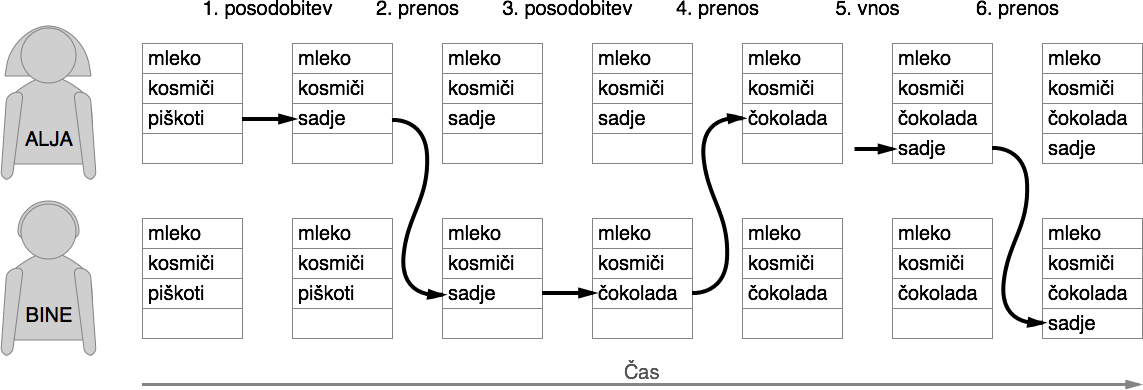
\includegraphics[width=16cm]{problem1.png}
\end{center}
\caption{Diagram sočasnega urejanja nakupovalnega listka, pri čemer mora Alja dvakrat vpisati svojo željo po sadju.}
\label{problem1}
\end{figure}

Pri tako fleksibilni interakciji lahko nastane konflikt. Alja bi lahko spremenila piškote v sadje sočasno kot bi Bine spremenil piškote v čokolado. Oba bi svoje spremembe videla takoj. Vendar spremembe Alje potrebujejo nekaj časa, da pridejo do Bineta. Tudi spremembe Bineta potrebujejo nekaj časa, da pridejo do Alje. Ta zamuda lahko spremeni vrstni red Aljine in Binetove spremembe, kar povzroči nakonsistentnost kot je to prikazano na Sliki \ref{problem2}. Alja in Bine bi morala pri sebi imeti vedno enake artikle na nakupovalnem listku.

\begin{figure}[placement h]
\begin{center}
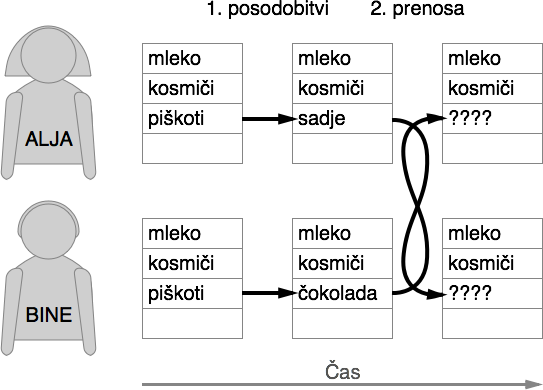
\includegraphics[width=8cm]{problem2.png}
\end{center}
\caption{Diagram sočasnega urejanja nakupovalnega listka. Vprašaji v zadnjem koraku pomenijo, da je seznam v konfliktu in mora biti razrešen, da zagotovimo konsistentnost. }
\label{problem2}
\end{figure}

\pagebreak

Predstavljajmo si enostavno rešitev za posodabljanja nakupovalnega listka, ki Alji in Binetu pokaže vedno zadnjo spremembo, ki je bila narejena na seznamu. Alja bi piškote spremenila v sadje, nato pa bi prišla Binetova sprememba v čokolado. Na drugi strani je Bine piškote spremenil v čokolado, nato pa bi sprejel Aljino sadje. V tem primeru bi Alja in Bine na koncu imela dva različna seznama, česar sploh ne bi opazila. Primer slabega reševanja konfliktov je prikazan na Sliki \ref{problem3}.

\begin{figure}[placement h]
\begin{center}
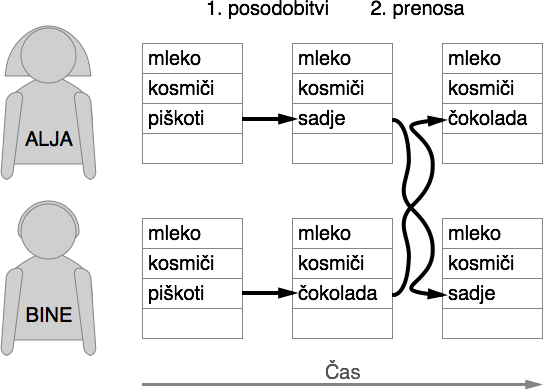
\includegraphics[width=8cm]{problem3.png}
\end{center}
\caption{Diagram sočasnega urejanja nakupovalnega listka. Konflikt v zadnjem koraku je rešen na način, da Alja in Bine sprejmeta zadnjo narejeno spremembo. Rešitev je slaba, saj ne zagotavlja konsistentnosti. }
\label{problem3}
\end{figure}

Problem nastane še večji pri sodelovanju večih uporabnikov in še z večjo zamudo pri dostavi sprememb na nakupovlnam listku. Recimo, da se Alji in Binetu pridruži še Cene. Bine ima počasen internet. Alja in Cene na seznam dodata in odstranita deset novih artiklov še preden Bine dobi eno spremembo. Medtem ko Bine ureja svoj seznam, so spremembe Alje in Ceneta še na poti k njemu. Za zagotovitev konsistentnosti bi morala aplikacija upoštevati zakasnjene oddaljene spremembe na osnovi prvotne verzije nakupovalnega listka.

%%%%%%%%%%%%%%%%%%%%%%%%%%%%%%%%%%%%%%%%%%%%%%%%%%%%%%%%%%%%%%%%%%%%%%%%%%%%%%%%%%%%%%%%%%%%%%%%%%%%%%%%%%%%%%%%%%
\chapter{Sodelovanje v realnem času}

Kako reševati konflikte in zagotoviti konsistentnost med oddaljenimi uporabniki pri sočasnem urejanju, je eden izmed glavnih izivov moje diplomske naloge. V tem poglavju bomo raziskali protokole, ki omogočajo sodelovanje uporabnikov v realnem času in teoretično rešujejo omenjena problema. Najbolj razširjeni so Operativna transformacija (ang. Operational transformation), Diferenčna sinhronizacija (ang. Differential synchronization) in protokol Brez operativne transformacije (ang. Without operational transformation, bolj znan pod kratico WOOT).

%%%%%%%%%%%%%%%%%%%%%%%%%%%%%%%%%%%%%%%%%%%%%%%%%%%%%%%%%%%%%%%%%%%%%%%%%%%%%%%%%%%%%%%%%%%%%%%%%%%%%%%%%%%%%%%%%%
\section{Diferenčna sinhronizacija}
\label{sec:ds}

Konceptualno enostavni načini sinhronizacije so zaklepanje (ang. locking), prenašanje dogodkov (ang. event passing) in trosmerno združevanje (ang. three way merge).

\begin{description}
	\item[Zaklepanje] je najenostavnejši način. Ko uporabnik odpre skupni dokument, se mu dodeli pravica lasnika (ang. ownership). Le on ga lahko ureja. Vsi ostali uporabniki lahko v tistem času dokument gledajo (ang. read-only access). Cilj je delno dosežen. Vsi uporabniki imajo sinhroniziran dokument, vendar urejanje dokumenta se ne izvaja v realnem času. Izboljšava zaklepanja je delno zaklepenje pri katerem se uporabniku dodeli pravica lastnika le za majhen del dokumenta. Ta način ni najboljši kadar imajo uporabniki slabo povezavo. Paket z informacijo o zaklepanju in odklepanju se lahko izgubi. V dokumentu lahko nastanejo deli nad katerimi ima lahko več uporabnikov pravico lastnika. Pojavijo se tudi druga anomalije.
	\item[Prenašanje dogodkov] temelji na zaznavanju vseh interakacij, ki jih naredi uporabnik z urejevalnikom. V teoriji je to enostavno, saj vsak sistem omogoča zaznavanja tipkanja. V praksi je težko izvedljivo. Poleg tipkanja lahko uporabnik naredi tudi akcije kot so izreži besedilo, prilepi besedilo, povleci in spusti besedilo, zamenjava besedila... Akciji kot sta samodokončanje in pravpisni popravek lahko naredi tudi sam urejevalnik. Kaj narediti v teh primerih? Težava je tudi v tem, da lahko zaradi neke napake ali zamude v komunkaciji pride do dveh popolnom različnih dokumenetov, ki jih ne moremo poenotiti.
	\item[Trosmerno združevanja] uporabljajo programerji pri delu na skupnem projektu. Je zelo robusten sistem. Sestavljen je iz treh korakov. Uporabnik najprej svojo vsebino pošlje na strežnik. Strežnik izvzame narejene spremembe in jih združi s spremembami drugih uporabnikov. Nova kopija dokumenta se sinhronizira vsem uporabnikom. Sistem trosmernega združevanja ima nekaj slabosti. Če uporabnik naredi spremembo na dokumentu medtem, ko je sinhronizacija v teku, mora zavreči vse na novo narejene spremembe. Slabost je, da uporabnik ne dobi nobene povratne informacije (ang. feedback) med tipkanjem. Način trosmernega združevanja bi pri urejanju v realnem času deloval le v dveh primerih. Če bi si lahko privoščili, da bi uporabnika blokirali in sinhronizirali z novo verzijo na strežniku ali pa v primeru, da bi uporabnika sinhronizirali, ko neha tipkati. Ampak nobena od teh dveh variant ni urejanje dokumenta v realnem času.
\end{description}

Ker sinhronizacija in ohranjanje konsistentnosti med uporabniki ni enostavna, si oglejmo rešitev imenovano Diferenčna sinhronizacija (v nadaljevanju DF). DF je simetričen algoritem, ki uporablja neskončno ciklov razlik na dokumentih in z njimi popravlja ostale dokumente v ciklu. Najprej bomo preučili osnovno topologijo DS, ki teoretična podlaga za izboljšave z metodo dveh senc in z metodo garantirane dostave.

\subsection{Osnovna topologija}

Na Sliki \ref{ds1} je z diagramom prikazan DS. V osnovni topologiji obstajata dokument uporabnika in dokument računalnika. Oba sta locirana na istem sistemu brez internetne povezave. Med njima se nahaja dokument imenovan skupna senca (ang. common shadow). Predvidimo, da imajo na začetku vsi trije dokumenti isto vsebino. Cilj je, da so dokumenti vseskozi čim bolj enaki. Ostale entitete so še razlika, sprememba in popravek. Razlika je signal, ki pove, da se dokument uporabnika razlikuje od skupne sence. Na ta način vemo, da je uporabnik naredil spremembo na svojem dokumentu. Ni nam potrebno spremljati vsake uporabnikove akcije. Ko se ve, kakšne spremembe so bile narejene, se mora dokument prekopirati v senco. Sprememba se pošlje v smeri računalnika. Na dokumentu računalnika se naredi popravek. Proces se ponovi še v smeri računalnika proti uporabniku. Vsi trije dokumenti so sinhronizirani.

Sistem je zanesljiv. Težava je, da taka zasnova ne omogoča sodelovanja oddaljenih uporabnikov v realnem času saj vse skupaj poteka na enem sistemu.

\begin{figure}[placement h]
\begin{center}
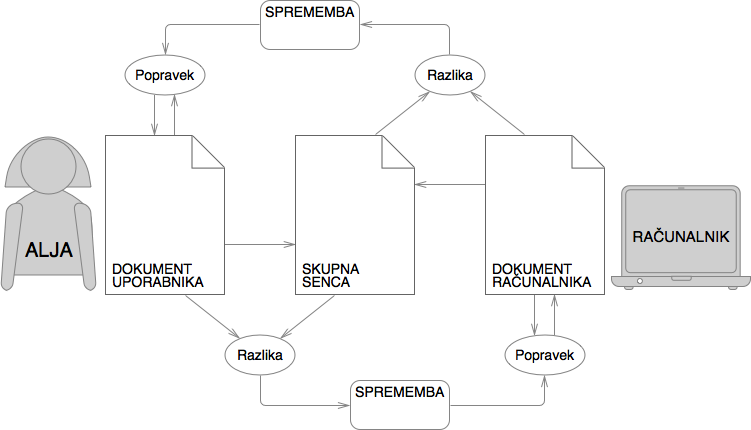
\includegraphics[width=9.2cm]{ds1.png}
\end{center}
\caption{Osnovna topologija Diferenčne sinhornizacije.}
\label{ds1}
\end{figure}

\subsection{Metoda dveh senc}

Konceptualno še vedno ostajamo pri istem algoritmu. Razlika je v topologiji. Namesto skupne sence uporabimo senco uporabnika in senco strežnika, ki se s popravki posodabljata ločeno. Taka zasnova DF omogoča sodelovanje oddaljenih uporabnikov. Vsak uporabnik je na svojem sistemu. Uporabnike povezuje centralni strežnik. Zaradi enostavnosti razlage je na Sliki \ref{ds2} prikazan le en uporabnik in strežnik, ki sta ločna s črtkano črto. Po vsakem ciklu morata biti dokument uporabnika in dokument strežnika identična.

Predvidimo, da se na začetku vsi dokumenti v konsistentnem stanju. Uporabnik začne tipkati. Vključi se signal, da je med dokumentom in senco uporabnika razlika. Ko se ve, kakšne spremembe so bile narejene, se mora dokument prekopirati v senco. Sprememba se pošlje strežniku. Na strežniku se naredita dva popravka, na senci in na dokumentu. Pomembno je, da se popravek na senci izvede brez problemov. Na dokumentu se naredi nejasen (ang. fuzzy) popravek. Nejasen popravek izvira iz sodelovanja med uporabniki. Če eden izmed uporabnikov naredi korenito spremembo na dokumentu, povzroči, da se popravek prvega uporabnika ne umesti v dokument tako kot bi si on želel. Nepredvideno stanje se reši v naslednji polovici cikla. Senca in dokument strežnika sta v tem trenutku različna. Ko se ve, kakšne so spremembe med senco in nepredvidenim dokumentom strežnika, se mora dokument prekopirati v senco. Sprememba se pošlje uporabniku. Ker je bila sprememba dokumenta strežnika narejena na podlagi sence strežnika, ki je bila ista kot senca in dokument uporabnika, se brez težav naredi popravek na senci in na dokumentu uporabnika. Dokumenti so sinhronizirani.

Sistem omogoča sodelovanje oddaljenih uporabnikov, vendar ni zanesljiv. Lahko se zgodi, da uporabnik na nezanesljivi povezavi od strežnika ne dobi nobenega odgovora. Do izgube spremembe lahko pride v prvem ali v drugem delu cikla. Senca uporabnika in senca strežnika nista več sinhronizirani. Edina rešitev za povrnitev nastalega stanje je, da povozimo uporabnikove spremembe. Tega si nihče ne želi.

\begin{figure}[placement h]
\begin{center}
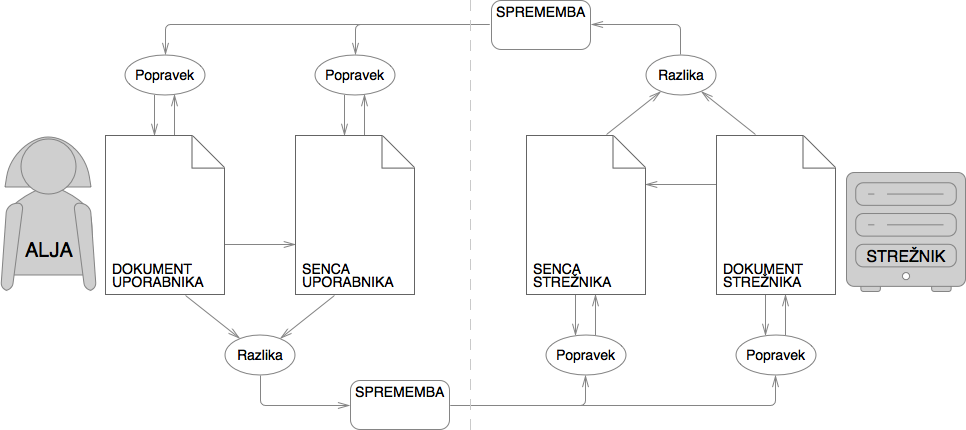
\includegraphics[width=11.83cm]{ds2.png}
\end{center}
\caption{Diferenčna sinhronizacija z metodo dveh senc.}
\label{ds2}
\end{figure}

\subsection{Metoda garantirane dostave}

DS z metodo garantirane dostave je nadgradnja metode dveh senc. Iz Slike \ref{ds3} lahko razberemo, da se je topologija razširila še z varnostnima kopijama sence uporabnika in sence strežnika. Tudi tokrat mora biti vseh šest dokumentov v konsistentnem stanju. Namesto ene same spremembe, se lahko pošlje več sprememb na enkrat. Nove v topologiji so tudi številke verzij. S črko {\tt n} je označena številka verzija uporabnika. S črko {\tt m} je označena številka verzija strežnika. Na začetku sta obe številki verziji enaki {\tt 0}.

\begin{figure}[placement h]
\begin{center}
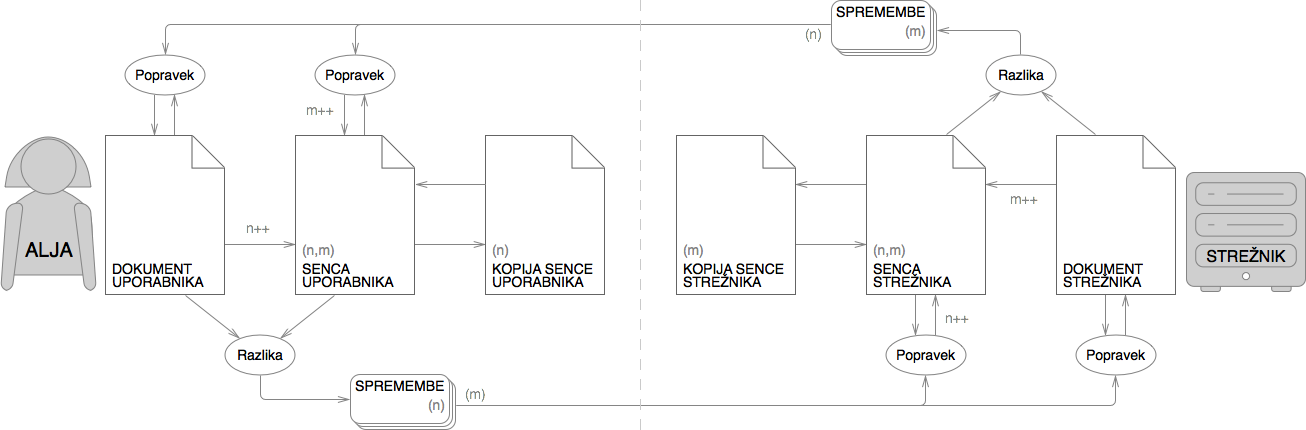
\includegraphics[width=16cm]{ds3.png}
\end{center}
\caption{Diferenčna sinhronizacija z metodo garantirane dostave.}
\label{ds3}
\end{figure}

Delovanje DS z metodo garantirane dostave bomo razložili na primeru. Na začetku je v vseh dokumentih beseda {\tt avto}. Alja v svoj dokument dopiše {\tt mobil}. Posledica razlike dokumenta uporabnika od sence uporabnika je sprememba {\tt mobil}. K sami spremembi se shrani številke verzije uporabnika na podlagi katere je bila sprememba osnovana. V seznam sprememb se torej shrani {\tt \{ +mobil;n=0 \}}. V tem trenutku se dokument Alje prekopira v njeno senco ter poveča se številka verzije uporabnika na {\tt n=1}. Sprememba se pošlje strežniku. Poleg spremembe se strežniku pošlje tudi številka zadnje sinhronizirane verzije strežnika {\tt m=0}. Stanje je prikazano na Sliki \ref{ds4}.

\begin{figure}[placement h]
\begin{center}
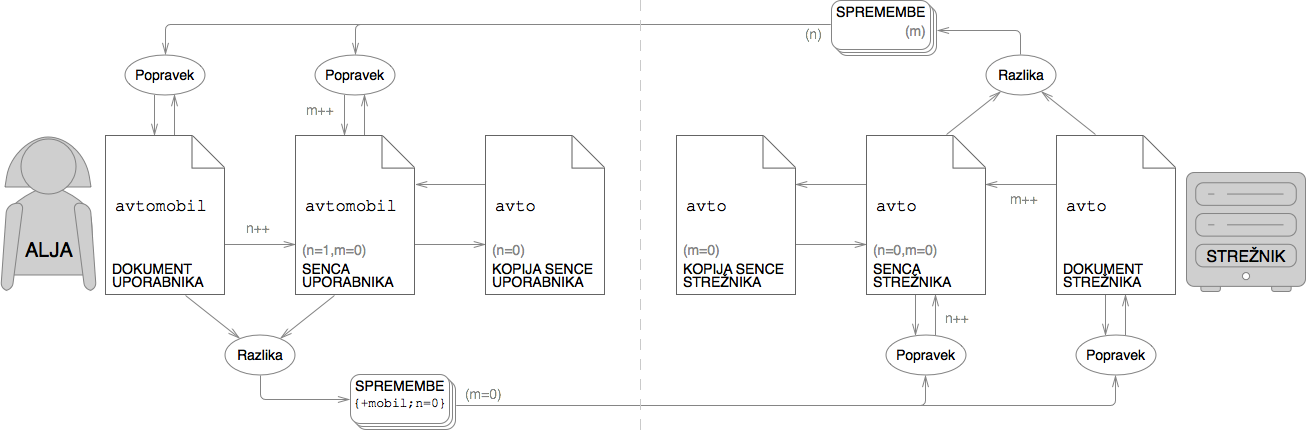
\includegraphics[width=16cm]{ds4.png}
\end{center}
\caption{Alja v svojem dokumentu vidi besedo avtomobil.}
\label{ds4}
\end{figure}

Strežnik primerja številki verzije uporabnika in strežnika spremembe s številkami verzije uporabnika in strežnika v senci strežnika (glej Sliko \ref{ds4}). Številki {\tt n} in {\tt m} sta v obeh primerih {\tt 0}, kar dovoljuje, da se naredi popravek na senci strežnika. Številka verzije uporabnika v senci strežnika se poveča na {\tt n=1}. Senca strežnika in senca uporabnika imata enako besedilo in enaki številki {\tt n} in {\tt m}, kar pomeni, da sta sinhronizirani. To se vidi tudi na Sliki \ref{ds5}. Popravek se naredi tudi na dokumentu strežnika, kar povzroči, da se senca strežnika prekopira v varnostno kopijo sence strežnika. Zakaj je to potrebno, bomo videli v nadaljevanju.

\begin{figure}[placement h]
\begin{center}
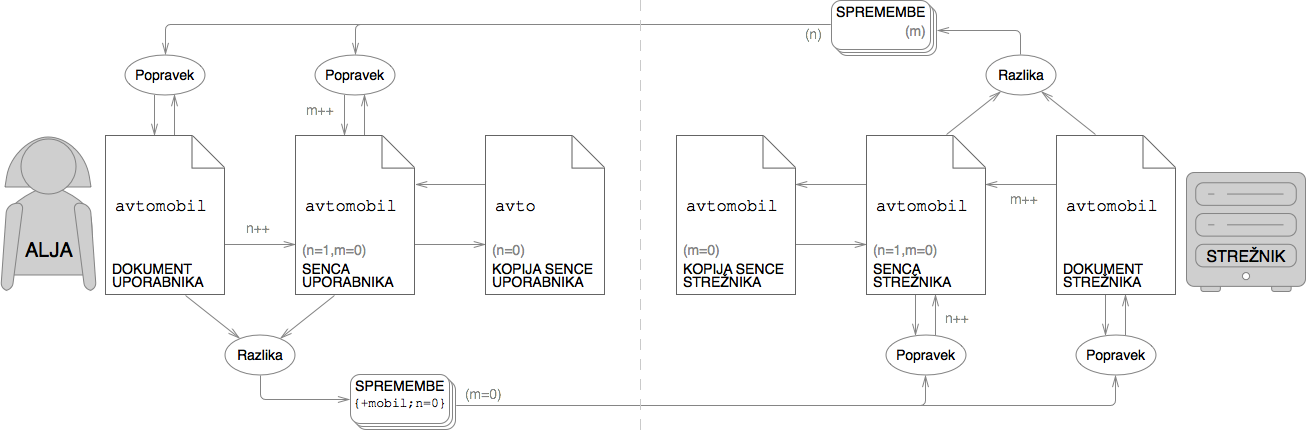
\includegraphics[width=16cm]{ds5.png}
\end{center}
\caption{Polovica cikla je končanega. Senci sta konsistentni.}
\label{ds5}
\end{figure}

Recimo, da uporabnik Bine na začetek dokumenta vpiše besedo {\tt Moj}. Na isti način kot Aljina sprememba se tudi njegova sprememba sinhronizira v dokument strežnika. Vsebina dokumenta strežnika je tako {\tt Moj avtomobil}. Sedaj lahko nadaljujemo z drugim delom cikla iz smeri strežnika proti Alji.

\begin{figure}[placement h]
\begin{center}
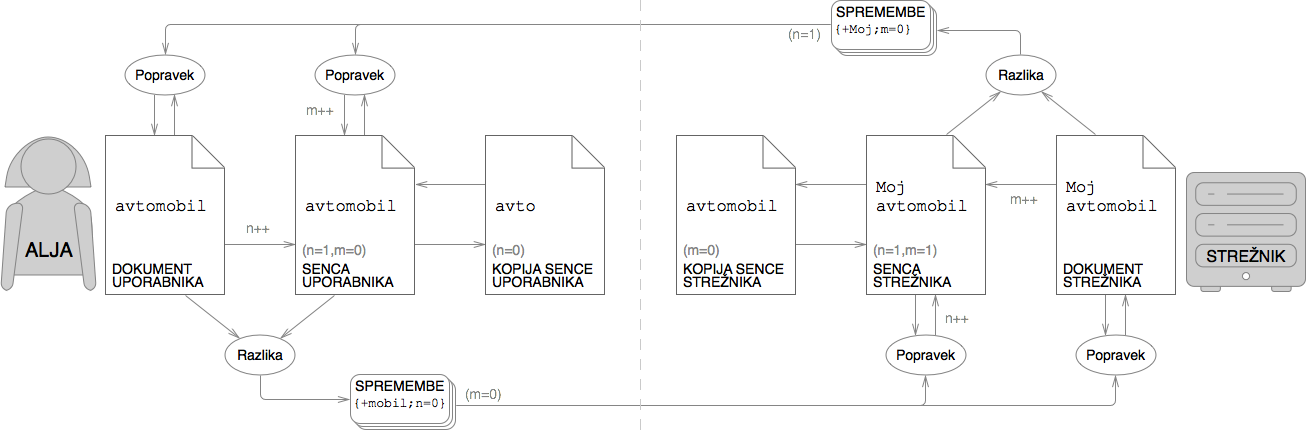
\includegraphics[width=16cm]{ds6.png}
\end{center}
\caption{Server prejme spremembo od Bineta, ki jo pošlje Alji.}
\label{ds6}
\end{figure}

Razlika dokumenta strežnika od sence strežnika je sprememba {\tt Moj} osnovana na številki verzije strežnika {\tt 0}. Sprememba {\tt \{ +Moj;m=0 \}} se pošlje k Alji. Poleg nje se pošlje tudi {\tt n=1} s katerim strežnik potrjuje, da je sprejel zadnjo Aljino spremembo. Pred tem se dokument strežnika prekopira v senco strežnika. Številka verzije strežnika {\tt m} v senci strežnika se poveča na {\tt 1}, Slika \ref{ds6}.

Zaradi slabe povezave Alja ne prejme sprememba {\tt \{ +Moj;m=0 \}} iz strežnika. Tega niti ne opazi, ampak tipka naprej. V svoj dokument doda klicaj. Ponovi se postopek podoben prvemu ciklu. K seznamu sprememb se doda {\tt \{ +!;n=1 \}}. Dokument Alje se prekopira v njeno senco, {\tt n} se poveča na {\tt 2}. Obe spremembi se pošljejo strežniku. Pomnimo, da za prvo spremembo Alja ni dobila nobenega odgovora. Številka zadnje sinhronizirane verzije strežnika je še vedno {\tt m=0}. Slika \ref{ds7} prikazuje nastalo situacijo.

\begin{figure}[placement h]
\begin{center}
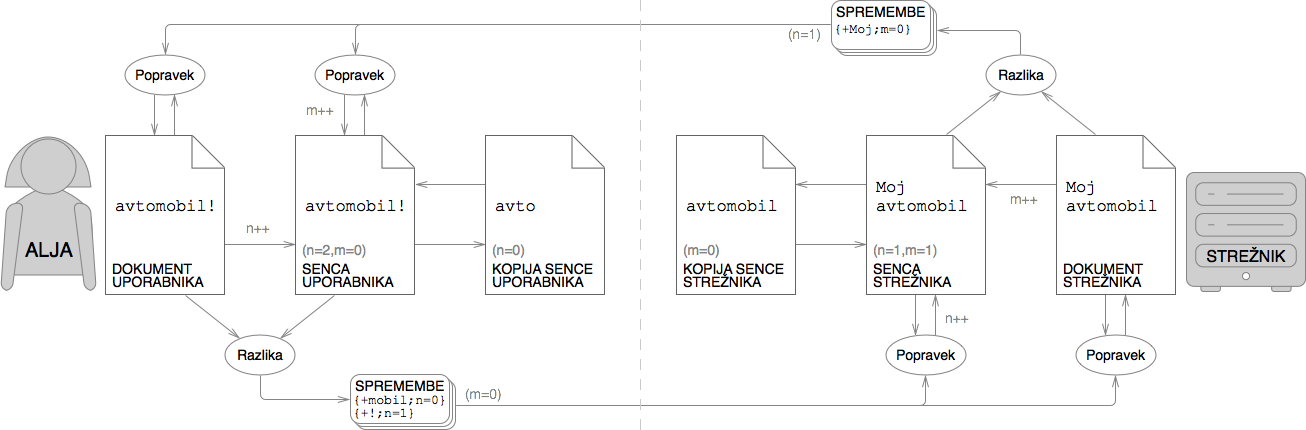
\includegraphics[width=16cm]{ds7.png}
\end{center}
\caption{Alja ni sprejela strežnikovih sprememb. V svojem dokumentu je naredila novo spremembo.}
\label{ds7}
\end{figure}

Strežnik sprejme Aljini spremembi. Najprej poskuša sprocesirati prvo spremembo {\tt \{ +mobil;n=0 \}}. Ker se številka zadnje sinhronizirane verzije strežnika {\tt m=0} ne ujema s številko verzije strežnika v senci strežnika, se sence strežnika povrne iz kopije sence strežnika (s številko {\tt m=0}) v katerem se nahaja {\tt avtomobil}. Strežnik poskusi ponovno sprocesirati prvo spremembo. Številki verzije strežnika {\tt m=0} se ujemajo. Številka verzije uporabnika je v prvi spremembi {\tt n=0}, v senci strežnika pa {\tt n=1}. To pomeni, da je strežnik v enem izmed prejšnjih ciklov že obdelal to spremembo, zato jo lahko ignorira. Strežnik nato poskusi sprocesirati drugo spremembo {\tt \{ +!;n=1 \}}. Številki {\tt n=1} in {\tt m=0} se tokrat ujemajo. Strežnik lahko naredi popravek na senci strežnika. Številka {\tt n} se poveča za {\tt 1} na {\tt n=2}. Popravek se nato naredi tudi na dokumentu strežnika, naredi pa se tudi kopija sence strežnika. Senca uporabnika in senca strežnika sta sinhronizirani.

Opomba! Ko se je naredila povrnitev kopije sence strežnika, se je seznam strežniških sprememb pobrisal. Spremembe v dokumentih in številkah {\tt n} in {\tt m} si oglejmo na Sliki \ref{ds8}.

\begin{figure}[placement h]
\begin{center}
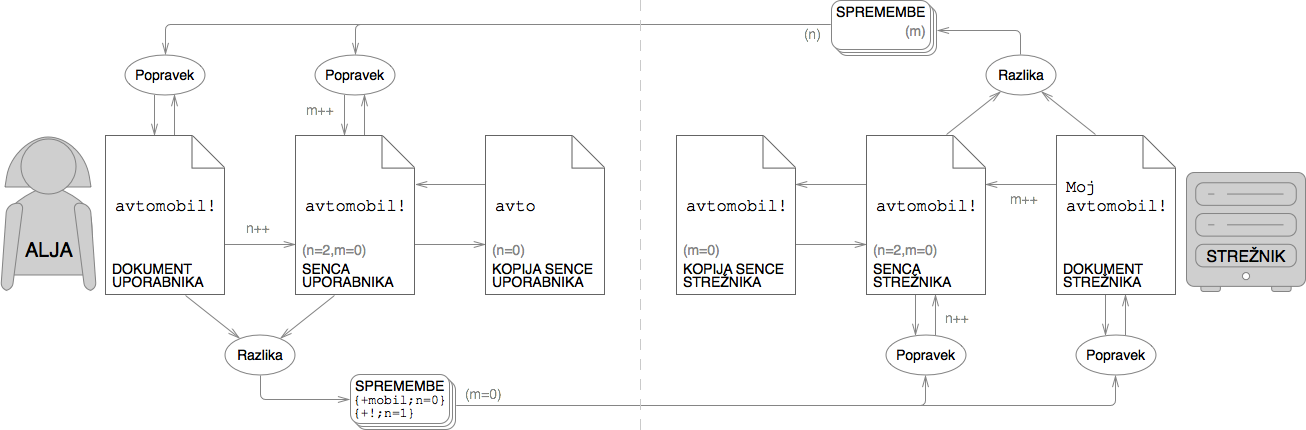
\includegraphics[width=16cm]{ds8.png}
\end{center}
\caption{Alja je strežniku poslala že dve spremembi.}
\label{ds8}
\end{figure}

Dokument strežnika in senca strežnika se na Sliki \ref{ds8} razlikujejta. Strežnik pogleda kakšne so spremembe na dokumentu. Tako kot v prvem ciklu najde spremembo \linebreak {\tt \{ +Moj;m=0 \}}. Sprememba se ponovno pošlje Alji. Tokrat je številka verzija uporabnika v senci dnevnika enaka {\tt 2}, zato se Alji poleg spremembe pošlje tudi {\tt n=2}. Še prej se dokument prekopira v senco in v senci strežnika se poveča številka verzije strežnika iz {\tt m=0} nazaj na {\tt m=1}.

Če bi bil strežnik spet neuspešen pri pošiljanju svojih sprememb, bi se seznam Aljinih sprememb povečeval vse dokler ne bi dobila odgovora od strežnika. Recimo, da tokrat strežniku uspe in Alja prejme spremembo {\tt \{ +Moj;m=0 \}}.

\begin{figure}[placement h]
\begin{center}
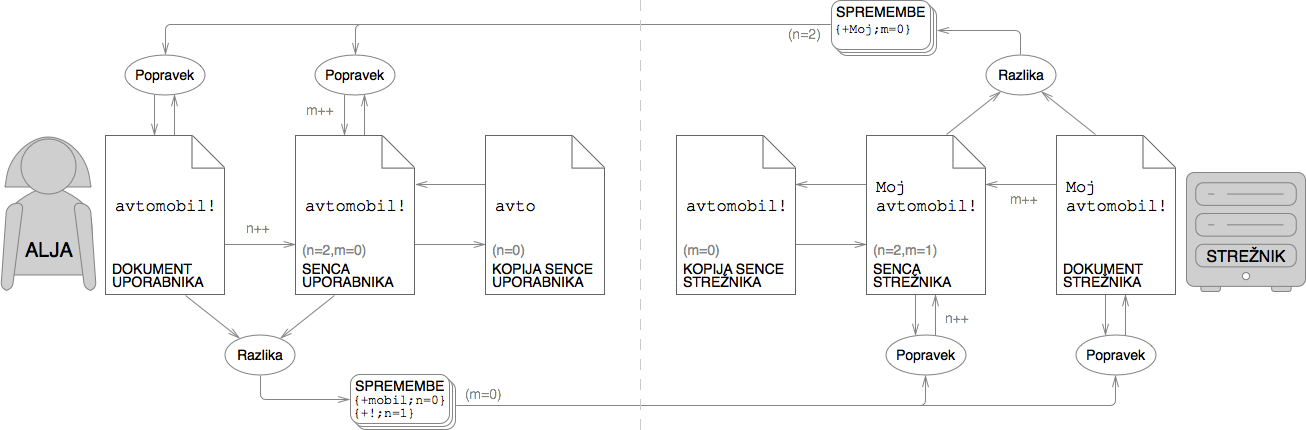
\includegraphics[width=16cm]{ds9.png}
\end{center}
\caption{Strežnik pošilja Alji potrditev njenih spremembe in spremembo Bineta.}
\label{ds9}
\end{figure}

Tokrat Alja primerja številke verzij. Številka verzije uporabnika v spremembi in v senci uporabnika je {\tt n=2}. Številka verzija strežnika v spremembi in v senci je {\tt m=0}. Sprememba je primerna za popravek na senci uporabnika. Naredijo se naslednje akcije. Na senci uporabnika se naredi popravek. Številka verzije zadnje sinhronizacije s strežnikom se v senci uporabnika poveča na {\tt m=1}. Popravek se naredi na dokumentu strežnika. Naredi se kopija sence uporabnika. Številka verzije uporabnika v kopiji sence uporabnika se poveča na {\tt n=2}. Ker je Alja uspešno sprejela potrditev strežnika, da je sprejel vse Aljine spremembe do številke verzije uporabnika {\tt n=2}, se iz seznama Aljinih sprememb pobrišejo vse spremembe, ki imajo številko verzije uporabnika manjše od {\tt 2} ({\tt n<2}).

\begin{figure}[placement h]
\begin{center}
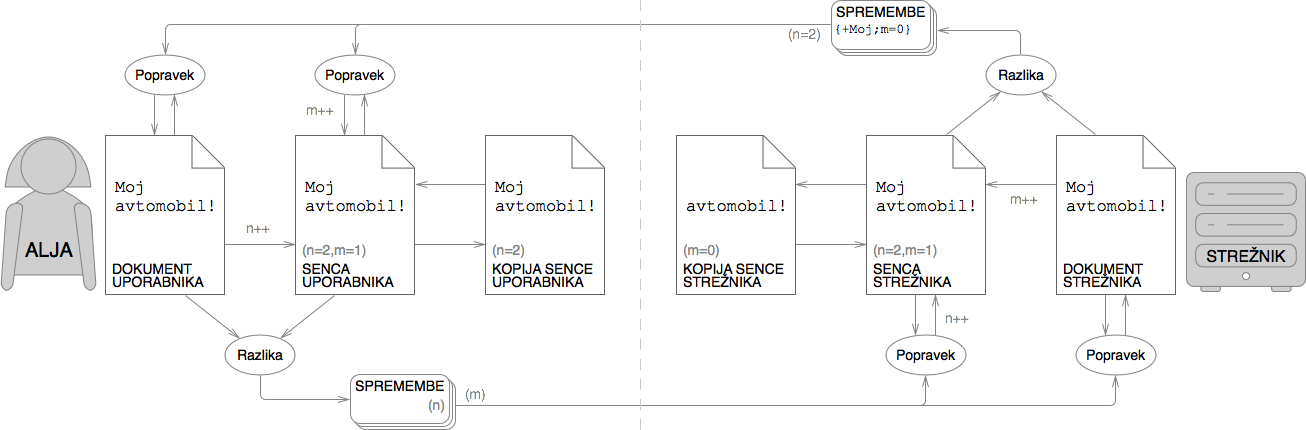
\includegraphics[width=16cm]{ds10.png}
\end{center}
\caption{Konsistentno stanje dokumentov.}
\label{ds10}
\end{figure}

Kjub temu, da je med sodelovanjem uporabnikov in strežnika prišlo do izpada v povezavi, so se dokumenti posinhronizirali. V dokumentu na koncu piše “{\tt Moj avtomobil!}”.

%%%%%%%%%%%%%%%%%%%%%%%%%%%%%%%%%%%%%%%%%%%%%%%%%%%%%%%%%%%%%%%%%%%%%%%%%%%%%%%%%%%%%%%%%%%%%%%%%%%%%%%%%%%%%%%%%%
\section{Operativna transformacija}
\label{sec:ot}

Operativna transformacija se je prvič omenjala v članku Concurrency Control in Groupware Systems. Pri Googlu so Operativno transformacijo vzeli za osnovno pri načrtovanju protokola Wave, ki se uporablja v Google Docsih, kar nakazuje na njeno uporabnost.

Zaradi razumljivosti bomo besedilo, ki ga urejajo uporabniki, poimenovali dokument. Dokument je shranjen kot serija kronoloških sprememb narejenih na dokumentu. Primer spremembe je {\tt \{ Vstavi ‘M’ @11 \}}, ki pomeni “v dokumentu na lokacijo 11 vstavi črko M” ali {\tt \{ Pobriši @3-7 \}}, ki pomeni “v dokumentu pobriši vse znake med lokacijo 3 in 7”. Obstajajo še druge vrste sprememb kot so oblikovanja besedila, zaklep odstavka, razveljevitev spremembe... Zaradi enostavnosti razlage se bomo osredotočili le na omenjena dva tipa sprememb. Ko uporabnik ureja besedilo, ne spreminja osnovnih znakov, ki bi skupaj predstavljali besedilo kot dokument. Namesto tega se njegove spremembe shranjujejo v revizijski dnevnik. Seveda dokumenta kot zaključene celote znakov obstaja. Vendar pomembne so spremembe, ki so bile narejene na tem dokumentu. Če se urejanju skupnega dokumenta pridruži nov uporabnik, mu iz revizijskega dnevnika ponovimo vse (od prve do zadnje) spremembe in že lahko sodeluje pri urejanju tako kot ostali uporabniki.

Glede na to, da poznamo revizijo vseh sprememb narejenih na dokumentu, lahko preverimo, kaj je uporabnik imel v svojem urejevalniku, preden je naredil novo spremembo. Na ta način njegovo spremembo pravilno umestimo v skupno besedilo skupaj z ostalimi spremembami, ki so bile narejene med tem. Algoritem, ki skrbi za umeščanje ali združevanje (ang. merging) sprememb, se imenuje Operativna transformacija (v nadaljevanju OT).

\bigskip

Poglejmo delovanje OT na primeru. Predpostavimo, da imamo dokument v katerem se trenutno nahaja stavek “ENOSTAVNO KOT PASULJ” in zasede dvajset lokacij. Urejanju tega dokumenta se pridružita Alja in Bine. Če Bine spremeni stavek v “ENOSTAVNO KOT KEKS”, potem je za to moral narediti pet sprememb.

\begin{figure}[placement h]
\begin{center}
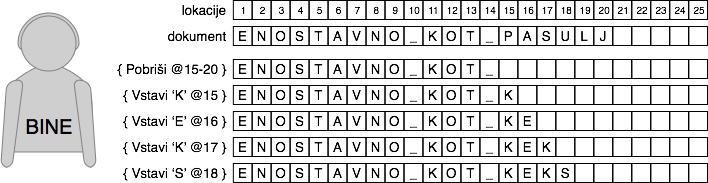
\includegraphics[width=12cm]{ot1.png}
\end{center}
\caption{Bine naredi pet sprememb.}
\label{ot1}
\end{figure}

Predstavljajmo si, da med tem ko Bine tipka, začne stavek spreminjati tudi Alja. in sicer v “TAKO ENOSTAVNO KOT PASULJ”. Tudi Alja je morala narediti pet sprememb.

\begin{figure}[placement h]
\begin{center}
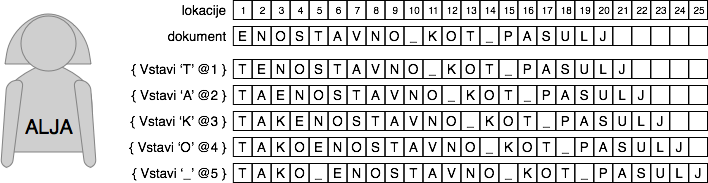
\includegraphics[width=12cm]{ot2.png}
\end{center}
\caption{Alja naredi pet sprememb.}
\label{ot2}
\end{figure}

Če bi Alja v naslednjem koraku naivno sprejela in izvršila Binetovo prvo spremembo, bi v stavku pobrisala napačne črke tako kot je to prikazano na Sliki \ref{ot3}.

\begin{figure}[placement h]
\begin{center}
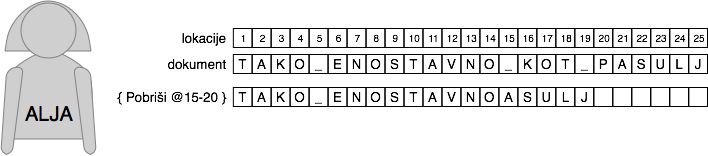
\includegraphics[width=12cm]{ot3.png}
\end{center}
\caption{Brez transformacije pride do nekonsistentnosti.}
\label{ot3}
\end{figure}

\pagebreak

Alja je imela pet znakov v začetku stavka, o katerih Bine še ni bil seznanjen. Lokacija Binetove spremembe je zato napačna glede na Aljino vezijo dokumenta. Da bi se izognili temu problemu, mora Alja narediti transformacijo Binetovih sprememb relativno na svoj lokalni dokument. V našem primeru, ko Alja sprejme Binetove spremembe, mora lokacijo spremembe zamakniti za pet znakov, kolikor jih je vpisala na začetku stavka. Ko naredi to transformacijo in izvrši Binetovo prvo spremembo, dobi pravilen stavek.

\begin{figure}[placement h]
\begin{center}
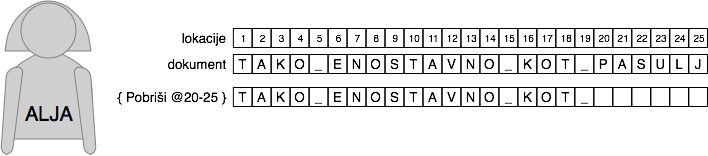
\includegraphics[width=12cm]{ot4.png}
\end{center}
\caption{Z uporabo Operativne transformacije dobimo pravilen rezultat.}
\label{ot4}
\end{figure}

Ko transformira in izvede še ostale štiri spremembe, dobi končno verzijo dokumenta.

\begin{figure}[placement h]
\begin{center}
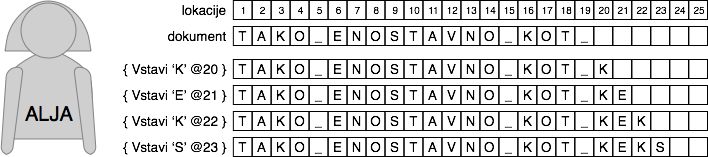
\includegraphics[width=12cm]{ot5.png}
\end{center}
\caption{Končna verzija dokumenta, ki ga vidi Alja.}
\label{ot5}
\end{figure}

Včasih spremembe ne povzročajo konfliktov in ni potrebe po transformaciji. Ko Bine prejme Aljine spremembe, ni potrebe po zamikanju lokacij. Bine mora izvesti Aljine spremembe točno take, kot jih je ona izvedla na svojem lokalnem dokumentu.

\begin{figure}[placement h]
\begin{center}
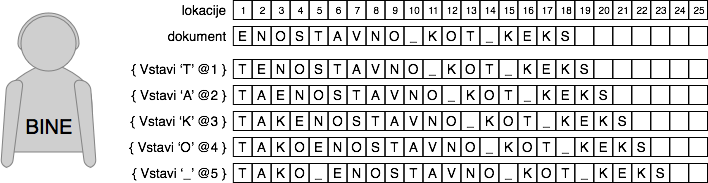
\includegraphics[width=12cm]{ot6.png}
\end{center}
\caption{Končna verzija dokumenta, ki ga vidi Bine.}
\label{ot6}
\end{figure}

Tako Alja kot Bine v svojem lokalnem dokumentu na koncu vidita stavek “TAKO ENOSTAVNO KOT KEKS”. Algoritem, ki smo ga uporabili za zamikanje sprememb, se imenuje Operativna transformacija. Pravilno implementiran algoritem nam garantira, da imajo vsi uporabniki, ko prejmejo vse spremembe, isto verzijo dokumenta.

%%%%%%%%%%%%%%%%%%%%%%%%%%%%%%%%%%%%%%%%%%%%%%%%%%%%%%%%%%%%%%%%%%%%%%%%%%%%%%%%%%%%%%%%%%%%%%%%%%%%%%%%%%%%%%%%%%
\subsection{Protokol sodelovanja}

Z uporabo OT smo se naučili, kako z zamikanjem lokacij sprememb večim uporabnikom dopustiti urejanje istega dokumenta brez konflikov. Še vedno pa obstaja težava, kako vsako spremembo pravilno združiti z drugimi spremembami, če se le te zgodijo istočano. Zagotoviti moramo, da vsak oddaljeni uporabnik ve, da obstajajo spremembe, ki morajo biti združene. Za to skrbi Protokol sodelovanja (ang. Collaboartion protocol). Tehnologiji OT in Protokol sodelovanja skupaj, znak za znakom, skrbita za sodelovanja v realnem času.

Zavedati se moramo, da za urejanje dokumenta v realnem času skrbijo tako strežnik kot odjemalci. Običajno so to spletni brskalniki uporabnikov. Pri urejanjeju dokumenta mora odjemalec sprocesirati vse spremembe, ki jih naredi uporabnik, in jih poslati na strežnik. Sprocesirati mora tudi vse spremembe drugih uporabnikov, ki mu jih pošlje strežnik. Seveda brez sodelovanja strežnika ne gre.

Najprej si oglejmo, katere podatke si morajo beležiti odjemalci in katere strežnik.

Vsak odjemalec si mora beležiti:
\begin{itemize}
	\item Številko zadnje sinhronizirane revizije. Na Sliki \ref{pc1} so označene s sivim krogcem in številko.
	\item Čakajoče spremembe. To so spremembe, ki so bile narejene v odjemalcu in niso še bile poslane na strežnik.
	\item Poslane spremembe. To so spremembe, ki so bile poslane na strežnik, vendar jih strežnik še ni potrdil.
	\item Trenutno stanje dokumenta kot ga vidi uporabnik.
\end{itemize}

Na strežniku se shranjujejo tri stvari:
\begin{itemize}
	\item Čakajoče spremembe. To so spremembe, ki jih je strežnik sprejel, a še ni sprocesiral.
	\item Revizijski dnevnik. Dnevnik v katerem je celotna zgodovina sprememb.
	\item Trenutno stanje dokumenta, kot bi ga morali v najkrajšem možnem času videti vsi uporabniki.
\end{itemize}

S hranjenjem in uporabo teh informacij je mogoče zasnovati komunikacijo med strežnikom in odjemalci tako, da so oddaljeni urejevalniki drug od drugega sposobni naglo sprocesirati spremembe.

Oglejmo si kako je v vzorčnem dokumentu poskrbljeno za komunikacijo med strežnikom in odjemalcem. Na Sliki \ref{pc1} zunanja stolpce predstavljata uporabnika Aljo in Bineta, ki urejata skupni dokument. Srednji stolpec je strežnik. Spremembe, ki jih naredita Alja in Bine in se pošljejo na strežnik, so označene v ovalni obliki. OT, ki smo jih spoznali v tem poglavju, bodo na naslednjih slikah označene s peterokotnikom.

Alja začne tipkati “V” na začetku dokumenta.

\begin{figure}[placement h]
\begin{center}
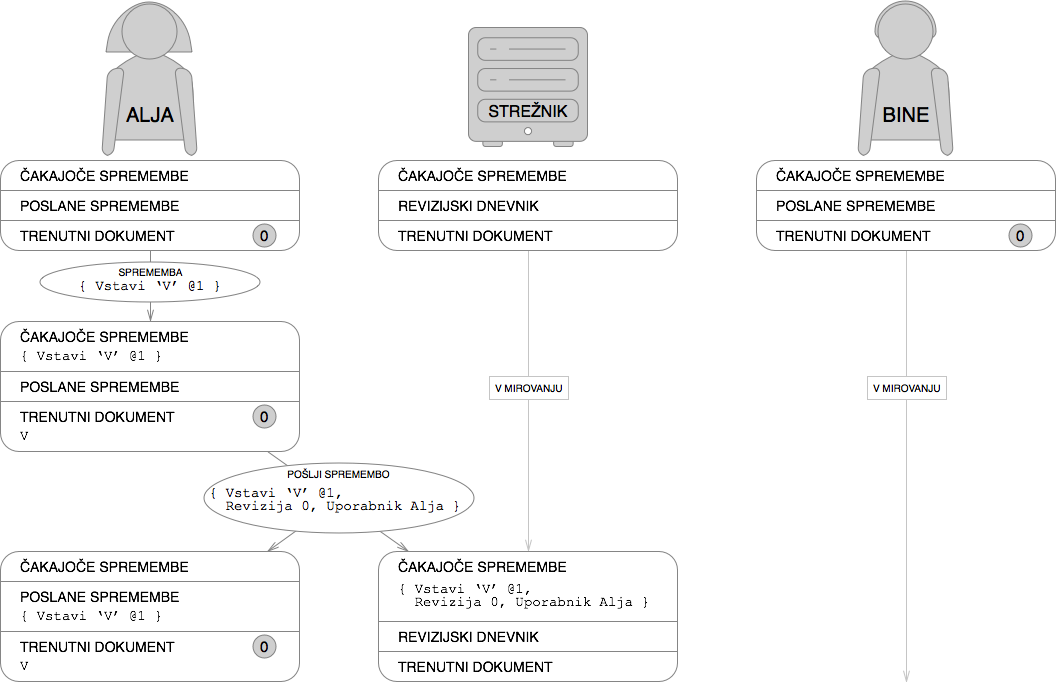
\includegraphics[width=14cm]{pc1.png}
\end{center}
\caption{Alja začne tipkati. Bine je v mirovanju.}
\label{pc1}
\end{figure}

Aljin urejevalnik si spremembo {\tt \{ Vstavi ‘V’ @1 \}} shrani med čakajoče spremembe. V naslednjem trenutku se le ta pošlje na server ter se prestavi na seznam poslanih sprememb. Poleg same spremembe, se strežniku pošlje tudi številka revizije in avtorja spremembe (uporabnika). Informacija o uporabniku je pomemba iz vidika avtentikacije. O številki revizije, bom več povedal v naslednjih korakih. Glej Sliko \ref{pc1}, strežnik sprejme Aljino prvo spremembo in jo doda med čakajoče spremembe.

Odjemalec lahko strežniku v enem pošiljanju pošlje tudi več črk za vstavljenje v dokument. Koliko črk se bo poslalo na enkrat je odvisno od implementacije urejevalnika in algoritma za zaznavanje sprememb. Več o tem v naslednjih poglavjih. Na Sliki \ref{pc2} vidimo, da Alja nadaljuje s tipkanjem in doda “ slogi ” v svoj urejevalnik. Alja v svojem trenutnem dokumentu vidi “V slogi ”. V istem času Bine vpiše “je moč!” v svoj prazen dokument. Ne pozabimo, da Bine še vedno ni prejel Aljinih sprememb.

\begin{figure}[placement h]
\begin{center}
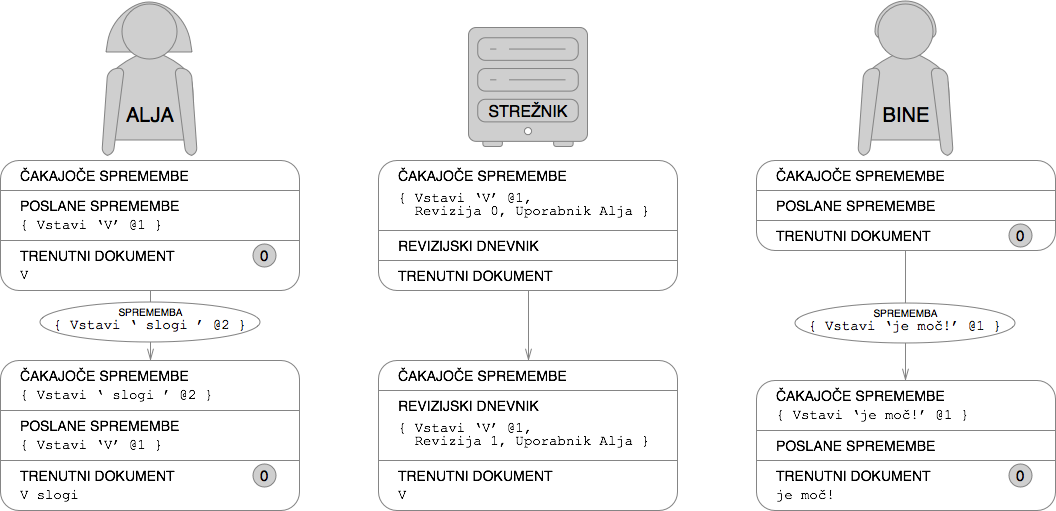
\includegraphics[width=14cm]{pc2.png}
\end{center}
\caption{Alja nadaljuje s tipkanjem. Bine na drugi strani tudi začne pisati na začetek svojega dokumenta. Strežnik o tem še ni obveščen.}
\label{pc2}
\end{figure}

Aljin {\tt \{ Vstavi ‘ slogi ’ @2 \}} je bil dodan med čakajoče spremembe in še ni poslan na strežnik. Pravilo je, da nikoli strežiku ne pošiljamo več kot ene čakajoče spremembe na enkrat. Dokler Alja od strežnika ne dobi potrditve prve spremembe, bo njen urejevalnik vse nove spremembe hranil med čakajočimi spremembami. Na Sliki \ref{pc2} lahko opazimo, da si je server Aljino prvo spremembo že shranil v revizijski dnevnik.

\pagebreak

V naslednjem koraku, kot je to prikazano na Sliki \ref{pc3}, strežnik Binetu pošlje Aljino prvo spremembo ter Alji odgovoril s potrditvijo, da si je zabeležil njeno spremembo v revizijski dnevnik.

\begin{figure}[placement h]
\begin{center}
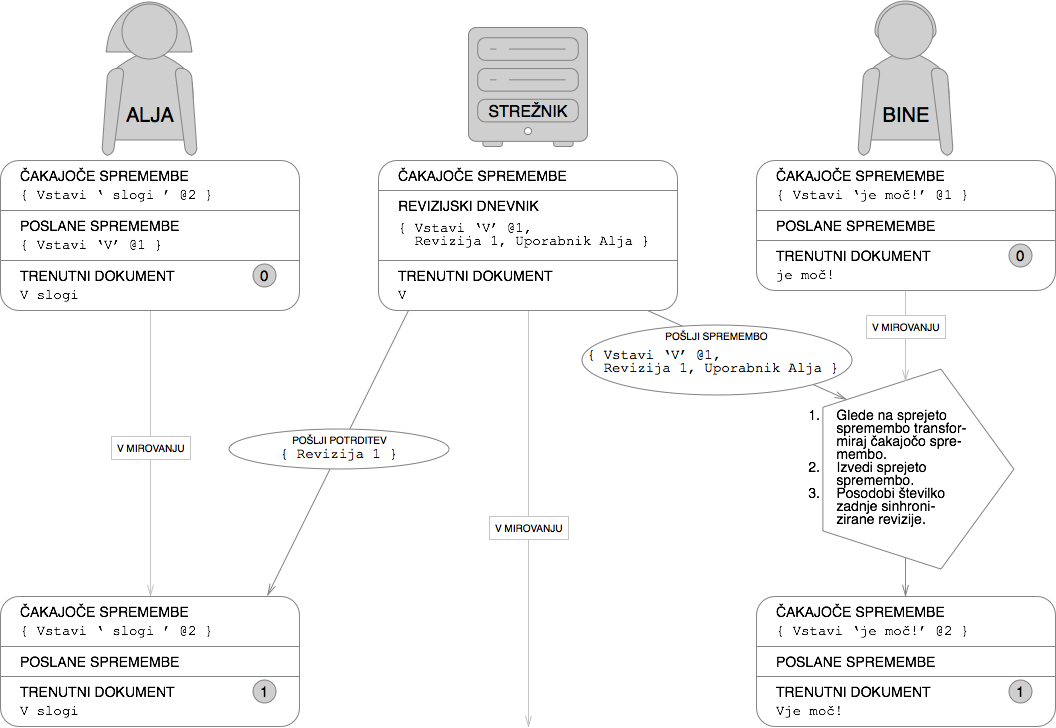
\includegraphics[width=14cm]{pc3.png}
\end{center}
\caption{Strežnik procesira Aljino prvo spremembo.}
\label{pc3}
\end{figure}

Bine sprejme Aljino spremembo od strežnika. Z uporabo OT mora transformirati svojo čakajočo spremembo {\tt \{ Vstavi ‘je moč!’ @1 \}}. Ker je Alja na začetek dokumenta že vpisala “V”, Binetov urejevalnik njegovo spremembo zamakne za eno lokacijo. Po tem procesu Binetov urejevalnik v trenutni dokument vstavi Aljino spremembo "V"\ in posodobi številko zadnje sinhronizirane revizije na 1. Alja je med tem sprejela potrditev iz strežnika. Tudi ona posodobi številko zadnje sinhronizirane revizije na 1. Svojo spremembo odstrani iz seznama poslanih sprememb.

V Aljinem trenutnem dokumentu se nahaj "V slogi ". V Binetovem trenutnem dokumentu se nahaj "Vje moč!", kar nakazuje, da še ni prejel vseh sprememb. Sledi pošiljanje čakajočih sprememb.

\pagebreak

Na Sliki \ref{pc4} se vidi, da oba uporabnika hkrati pošljeta spremembo, vendar strežnik sprejeme Aljino sprejme pred Binetovo in jo zato tudi sprocessira prej. Njeno spremembo iz seznama čakajočih sprememb prestavi v revizijski dnevnik. Pri tem mora le popraviti številko revizije, ki enolično označuje spremembo. Pomnimo, da je Alja pri pošiljanju svoje spremembe poslala številko zadnje sinhronizirane revizije, številko 1. Strežnik na ta način ve, da je njena sprememba narejena na podlagi prve revizije. Ker se v revizijski dnevnik pričakuje sprememba, ki je naslednja po vrsti, lahko njeno spremembo brez težav umesti v trenutni dokument.

\begin{figure}[placement h]
\begin{center}
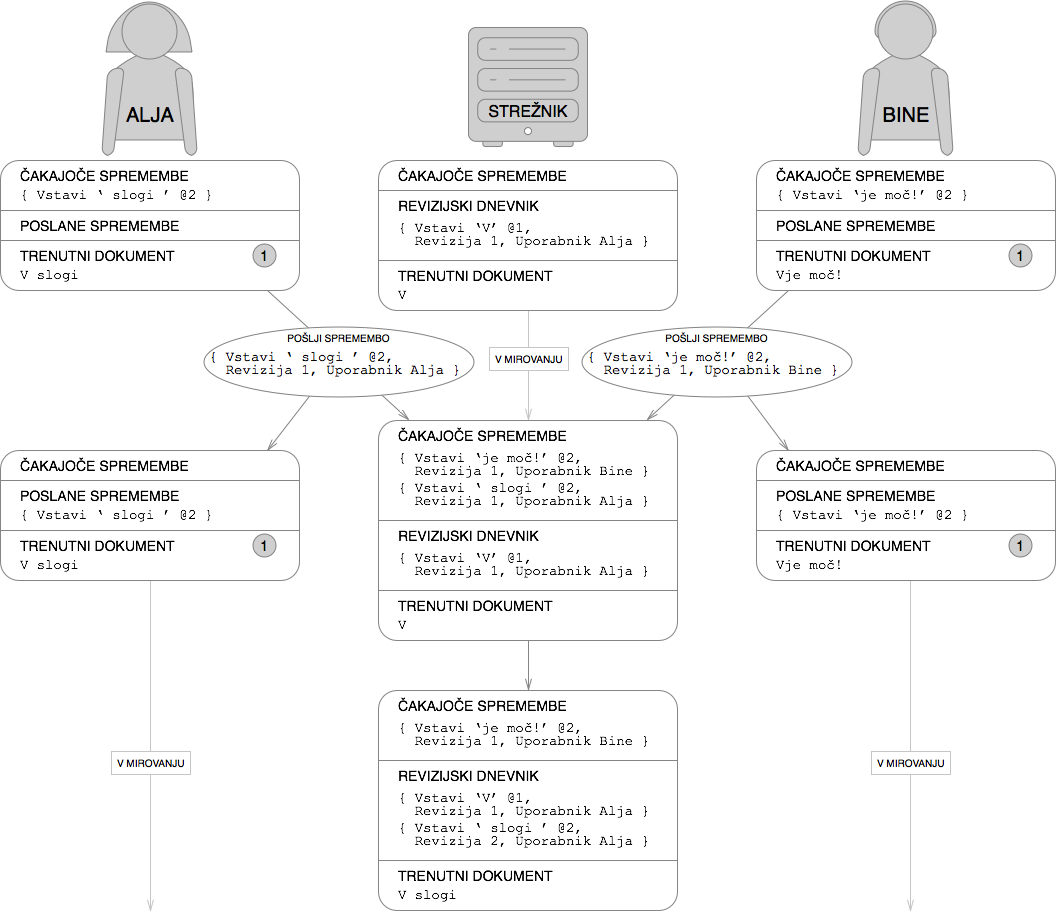
\includegraphics[width=14cm]{pc4.png}
\end{center}
\caption{Istočasno sodelovanje Aljinega in Binetovega urejevalnika preko strežnika.}
\label{pc4}
\end{figure}

Sledi potrditev spremembe Alji s številko revizije 2. Binetu se pošlje novo spremembo. Kot na Sliki \ref{pc3} se tudi v primeru na Sliki \ref{pc5} začne izvajati OT v Binetovem urejevalniku. Ker nima nobene čakajoče spremembe, ni potrebe po uporabi OT. Aljina sprememba se vstavi v njegov dokument brez transformacije. Številka zadnje sinhronizirane revizije se Binetu poveča na 2. Ker strežnik Alji odgovori s potrditvijo, se tudi njej poveča številka zadnje sinhronizirane revizije na 2.

\pagebreak

OT se ne dogaja samo pri odjemalcih, ampak je nujna tudi na strežniku. Zakaj bomo ugotovi kmalu. Med tem ko se odjemalca ukvarjata z zahtevami strežnika (potrditev pri Alji in sprememba pri Binetu), je strežnik začel procesirati Binetovo čakajočo spremembo {\tt \{ Vstavi ‘je moč!’ @2, Revizija 1, Uporabnik Bine \}}. Bine je v času pošiljanja spremembe (Slika \ref{pc4}) verjel, da bo njegova sprememba nosila zapredno številko revizije 2. Vendar strežnik je že obdelal Aljino spremembo, katero je v revizijski dnevnik zapisal kot drugo spremembo. V tem trenutku mora strežnik z uporabo OT transformirati Binetovo spremembo, da jo bo lahko shranil kot revizijo 3.

\begin{figure}[placement h]
\begin{center}
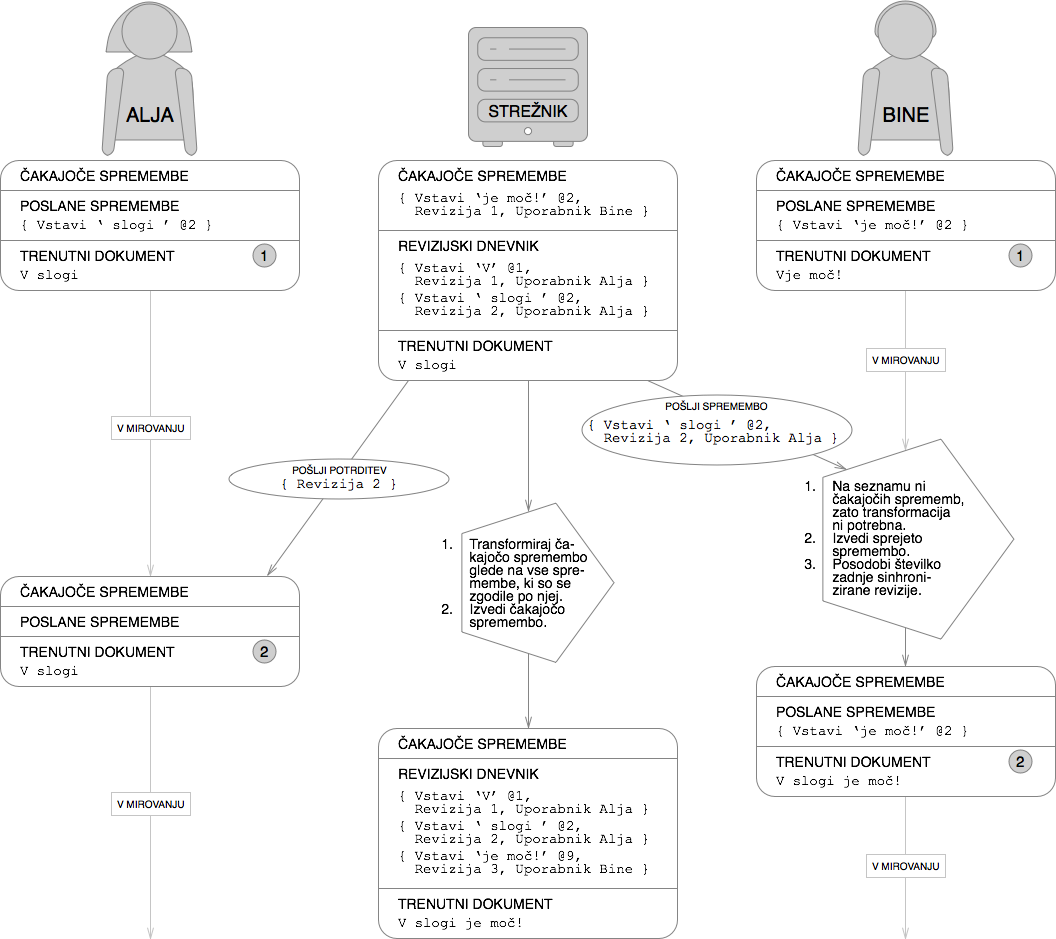
\includegraphics[width=14cm]{pc5.png}
\end{center}
\caption{Strežnik uporabi OT pri obdelovanju Binetove spremembe.}
\label{pc5}
\end{figure}

Binetovo spremembo transformira glede na spremembe, ki so bile storjene od kar je Bine zadnjič naredil sinhronizacijo s strežnikom. V našem primeru je bila narejena le Aljina sprememba {\tt \{ Vstavi ‘ slogi ’ @2 \}}, ki je povzročila zamik Binetove spremembe za 7 lokacij. Končna sprememba v revizijskem dnevniku izgleda kot {\tt \{ Vstavi ‘je moč!’ @9, Revizija 3, Uporabnik Bine \}}.

\pagebreak

Na koncu Bine dobi potrditev svoje spremembe in Alja prejme Binetovo spremembo. Številka zadnje sinhronizirane revizije se obema poveča na 3. V revizijskem dnevniku so 3 revizije. V tem tenutku imajo strežnik in oba urejevalnika isti dokument z vsebino “V slogi je moč!”. Glede na to, da uporabnika nimata več čakajočih sprememb je to tudi končna verzija dokumenta, ki sta ga skupaj uredila uporabnika Alja in Bine.

\begin{figure}[placement h]
\begin{center}
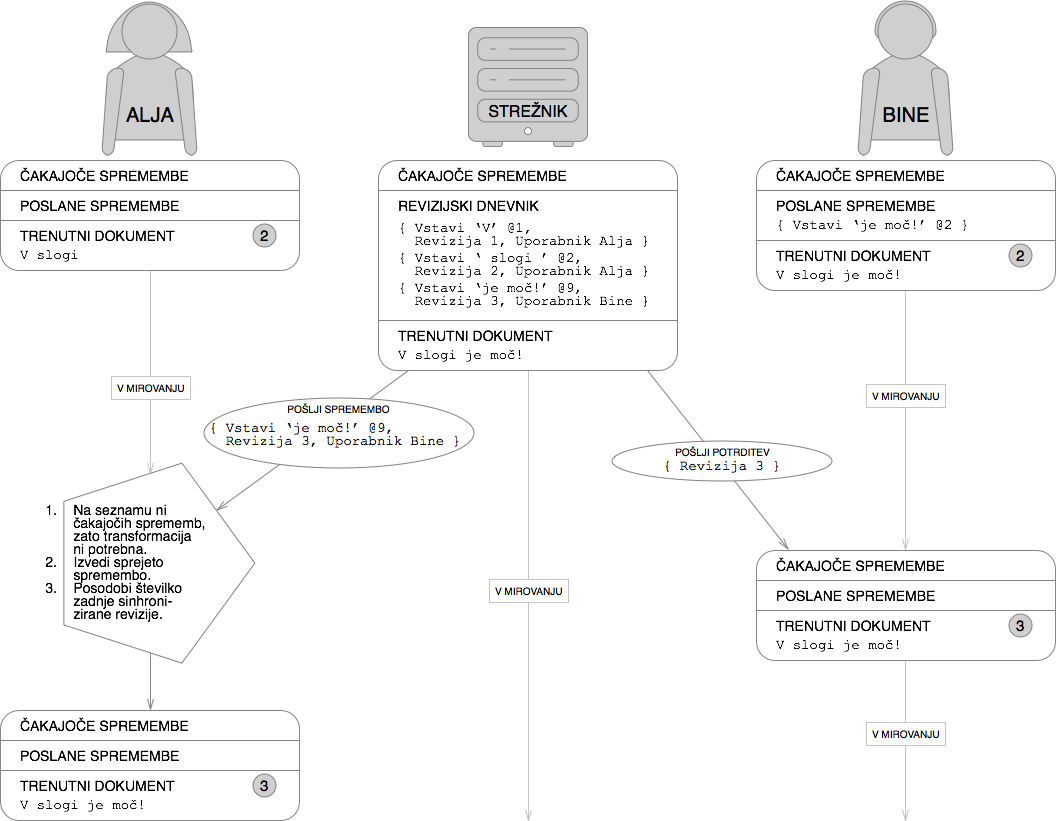
\includegraphics[width=14cm]{pc6.png}
\end{center}
\caption{Strežnik uporabi OT pri odelovanju Binetove spremembe.}
\label{pc6}
\end{figure}

%%%%%%%%%%%%%%%%%%%%%%%%%%%%%%%%%%%%%%%%%%%%%%%%%%%%%%%%%%%%%%%%%%%%%%%%%%%%%%%%%%%%%%%%%%%%%%%%%%%%%%%%%%%%%%%%%%
\section{Brez operativne transformacije}
\label{sec:woot}

V tem poglavju bomo opisali protokol Brez operativne transformacije, bolj znan pod kratico WOOT. Bil je narejen kot odgovor na kopleksnost OT. Rekli smo, da se \linebreak pri OT med uporabnike pošiljajo spremembe in lokacija sprememb, primer \linebreak {\tt \{ Vstavi ‘M’ @11 \}}. OT skrbi za pravilno transformacijo lokacij sprememb. Pristop WOOT je drugačen in ga je lažje razumeti. WOOT skrbi za pravilno razvrščanje sprememb oziroma operacij, kot se jih običajno poimenuje. Glavna razlika je v podajanju informacij. Lahko si predstavljamo, da na vsak znak v dokumentu kaže unikatni kazalec, to je identifikacijska številka. Med oddaljene uporabnike, ki sodelujejo pri urejanju dokumenta, se pošiljajo informacije med katerima znakoma oziroma na kateremu znaku je bila narejena sprememba. Posebnost protokola WOOT je, da se znakov v dokumentu nikoli ne briše, le označi se jih kot nevidne.

%%%%%%%%%%%%%%%%%%%%%%%%%%%%%%%%%%%%%%%%%%%%%%%%%%%%%%%%%%%%%%%%%%%%%%%%%%%%%%%%%%%%%%%%%%%%%%%%%%%%%%%%%%%%%%%%%%
\subsection{Podatkovni model}

Dokument pri WOOT-u je shranjen kot zaporedje znakov predstavljenih z identifikacijskimi številkami (ang. identifier order). Zaporedje znakov besedila “{\tt Ubogi mucek!}” se prikaže kot na Sliki \ref{woot1}.

\begin{figure}[placement h]
\begin{center}
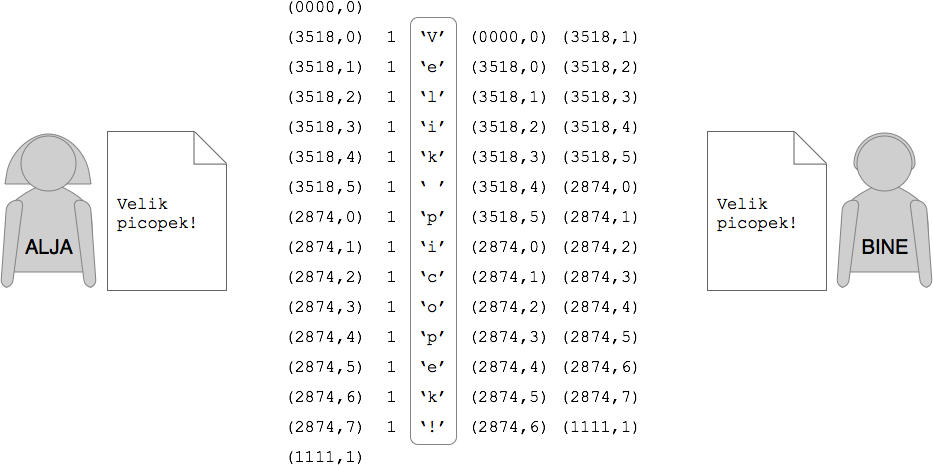
\includegraphics[width=9cm]{woot1.png}
\end{center}
\caption{Prikaz zaporedja znakov v dokumentu.}
\label{woot1}
\end{figure}

Za vsak znak v dokumentu hranimo 5 informacij: identifikacijo številko (ang. ID), vidnost, vsebino znaka, prejšnji znak in naslednji znak. Identifikacijska številka je kazalec na znak, ki je sestavljena iz unikatne oznake dokumenta in lokalne ure oziroma števca. Primer identifikacijske številka je {\tt (558,3)}. Unikatna oznaka dokumenta je številka, ki predstavlja uporabnika. Ko uporabnik prvič začne urejati dokument, se mu ta številka dodeli ali si jo izbere sam na podlagi predhodnega preverjanja unikatnostni. Lokalna ura je števec, ki se uporabniku povečuje za vsak vpisan znak. Na ta način je vsak znak v dokumentu označen z unikatnim kazalcem. Vidnost nam pove ali uporabnik določen znak vidi. Pri brisanju, se vidnost postavi na 0, sicer pa je vidnost pozitivna. Vsebina znaka je črka ali številka, ki jo znak predstavlja. Prejšnji znak je identifikacijska številka levega soseda. Naslednji znak je identifikacijska številka desnega soseda.

Poznamo tudi dva posebna znaka, ki označujeta konec in začetek dokumenta. Uporabljata se zato, da lahko prvemu znaku nastavimo prejšnjega in zadnjemu znaku naslednjega soseda. Alja in Bine na Sliki \ref{woot2} urejata dokument v katerem se trenutno nahaja besedilo “{\tt Ubogi mucek!}”. Dokument bi bil pri pri Alji in Binetu shranjen kot zaporedje znakov od {\tt U} do klicaja.

\begin{figure}[placement h]
\begin{center}
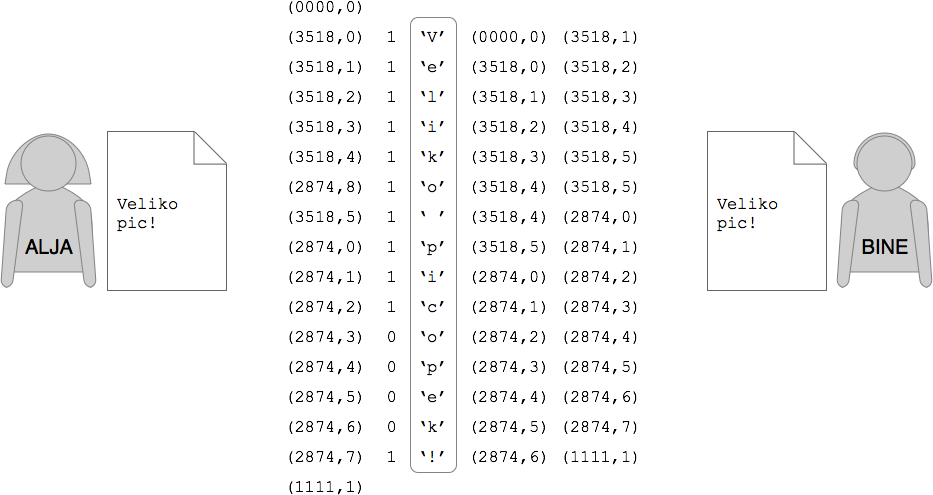
\includegraphics[width=13cm]{woot2.png}
\end{center}
\caption{Dokument shranjen po protokolu WOOT.}
\label{woot2}
\end{figure}

Znaka {\tt (00000)} in {\tt (11111)} označujeta začetek oziroma konec dokumenta. Za vse ostale znake se v stolpcih od leve proti desni hranijo identifikacijska številka, vidnost, vsebina, prejšnji ter naslednji soseda. Iz identifikacijskih številke vidimo, da je prvo besedo skupaj s presledkom napisala Alja z unikatno številko {\tt 217}. Drugo besedo skupaj s klicajem je napisal Bine. Njegov dokument je označen z unikatno števliko {\tt 558}. Lahko bi si vsak uporabnik shranjeval katera unikatna številka predstavlja katerega uporabnika, vendar ni potrebno. Vse črke so vidne. Nobena črka do sedaj še ni bila pobrisana. Glede na oznake sosedov so črke pravilne razvrščene.

%%%%%%%%%%%%%%%%%%%%%%%%%%%%%%%%%%%%%%%%%%%%%%%%%%%%%%%%%%%%%%%%%%%%%%%%%%%%%%%%%%%%%%%%%%%%%%%%%%%%%%%%%%%%%%%%%%
\subsection{Operacije}

Osredotočili se bomo na operaciji {\tt Vstavi} in {\tt Pobriši}. Ko uporabnik generira operacijo, se operacija najprej integrira lokalno. Nato se razpošlje vsem oddaljenim uporabnikom, ki sodelujejo pri urejanju. Ko jo sprejmejo, se še njim integrira v dokument.

Potreba po vnaprejšnji lokalni integracija pride iz razvrščanja znakov. Na primer, ko uporabnik generira spremembo {\tt \{ Vstavi ‘a’ @10 \}}, se le ta v uporabniškem vmesniku prikaže kot črka {\tt a} na lokaciji 10. Sprememba se mora pretvoriti v \linebreak {\tt \{ Vstavi ‘c’$\prec$‘a’$\prec$‘e’ \}}, ki pomeni vstavi črko {\tt a}, med črko {\tt c} in {\tt e}. Lokacija spremembe je tako definirana s svojima dvema sosedoma in ne s konkretno številko lokacije. Pretvorba je prikazana poenostavljeno. V dejanskem algoritmu bi sosednja dva znaka označlil z njunima identifikacijskama števikama. Podobno kot vstavljanje, se mora tudi brisanje pretvoriti WOOT protokolu primerno. Sprememba \linebreak {\tt \{ Pobriši @5 \}} pobriše znak na lokaciji 5. V primeru Alje in Bineta imamo na lokaciji 5 črko {\tt i}, zato moramo spremembo pretvoriti v {\tt \{ Pobriši ‘i’ \}}. Seveda je tudi ta primer poenostavljen, saj je tudi operacija brisanja vezana na identifikacijsko številko in ne na konkretno črko ali številko. Pomembno je poudariti, da znakov pri protokolu WOOT nikoli ne brišemo, ampak jih le skrivamo. Dokument je shranjen kot zaporedje uporabniku vidnih in uporabniku nevidinih znakov. Na ta način je razvrščanje spremembe vedno pravilno, saj je odvisno tudi od nevidnih znakov.

Alja in Bine želita stavek “{\tt Ubogi mucek!}” urediti v “{\tt Uboga muca!}”. Alja začne urejati drugo besedo in vstavi črko {\tt a}. Bine začne urejati prvo besedo in pobriše črko {\\ i}. Operaciji sta prikazani na Sliki \ref{woot3} in \ref{woot4}.

\begin{figure}[placement h]
\begin{center}
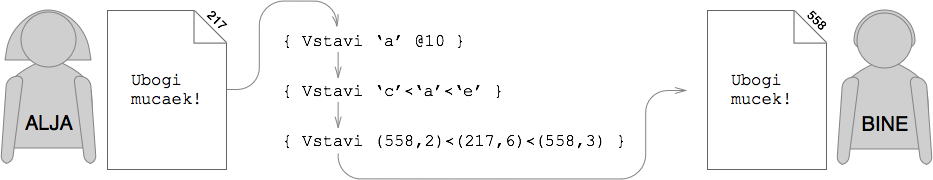
\includegraphics[width=13cm]{woot3.png}
\end{center}
\caption{Generiranje in integracija vstavljanja črke. Zadnji znak (presledek), ki ga je Alja vstavila (na Sliki \ref{woot2}), ima identifikacijska številka {\tt (217,5)}. Črka {\tt a} zatorej dobi številko {\tt (217,6)}. Vstaviti jo želimo na mesto med črko {\tt c} in {\tt e}, ki imata identifikacijski številki {\tt (558,2)} in {\tt (558,3)}.}
\label{woot3}
\end{figure}

\begin{figure}[placement h]
\begin{center}
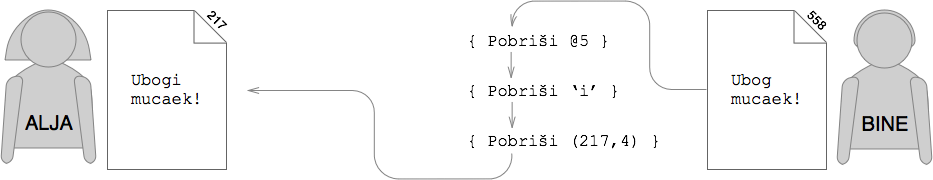
\includegraphics[width=13cm]{woot4.png}
\end{center}
\caption{Generiranje in integracija brisanja črke. Na Sliki \ref{woot2} vidimo, da je identifikacijska številka črke {\tt a} enaka {\tt (217,4)}. Operacija se pošlje Alji.}
\label{woot4}
\end{figure}

V naslednjem koraku Bine vstavi črko {\tt a} z identifikacijsko številko {\tt (558,6)} na podoben način kot je to naredila Alja na Sliki \ref{woot3}. Alja pa pobriše črki {\tt e (558,3)} in {\tt k (558,4)} v drugi besedi. Operacija je podobna kot na Sliki \ref{woot4}, ko to stori Bine. Končni stavek v dokumentu lahko vidimo na Sliki \ref{woot5}.

Čeprav so v dokumentu shranjene vse črke, ki sta jih napisala Alja in Bine, se njima v urejevalniku kažejo le črke, ki so označene kot vidne. Na Sliki \ref{woot5} opazimo še eno zanimivost. Črka {\tt c (558,2)} ima kot naslednjega soseda shranjeno črko {\tt e (558,3)}. Pravi naslednji sosed pa je v bistvu črka {\tt a (217,6)}. Ta pojav je normalen, ni napaka, je le posledica integracije vstavljanja.

\begin{figure}[placement h]
\begin{center}
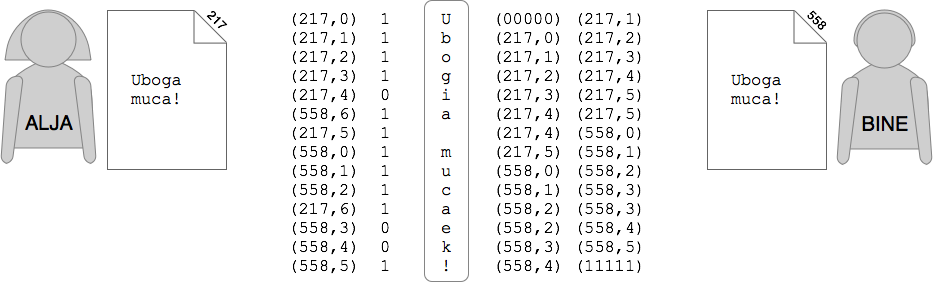
\includegraphics[width=13cm]{woot5.png}
\end{center}
\caption{Nekaj črk v dokumentu je skritih in jih Alja in Bine ne vidita.}
\label{woot5}
\end{figure}

V našem enostvanem primeru nismo omenjali čakalne vrste. Ko uporabnik sprejme operacijo, mora le ta iti najprej preko preverjanje predpogojev za izvršitev. Če predpogoj ni izpolnjen, se itegracija operacije začasno prestavi nazaj med čakajoče operacije. Primer, da pogoj ni izpolnjen je, ko uporabnik sprejme operacijo {\tt \{ Pobriši ‘M’ \}}, črka {\tt M} pa v njegovem dokumentu še ne obstaja. Operacija brisanja črke {\tt M} je prehitela vstavljanje črke {\tt M}. Operacija brisanja bo integrirana v naslednji iteraciji.

%%%%%%%%%%%%%%%%%%%%%%%%%%%%%%%%%%%%%%%%%%%%%%%%%%%%%%%%%%%%%%%%%%%%%%%%%%%%%%%%%%%%%%%%%%%%%%%%%%%%%%%%%%%%%%%%%%
\subsection{Točka-točka sodelovanje}

Protokola DS in OT omenjena v prejšnjih podpoglavjih temeljita na centralnih strežnikih in sta od njih odvisna. Za destribucijo vsebine so bolj učinkovita omrežja točka-točka (ang. peer-to-peer, kratica P2P). Ta potencial želimo izkoristiti tudi pri sodelovanju urejanja vsebine. Protokol WOOT je lahko implementiran popolnoma decentraliziran. Na primeru bomo videli, da ni odvisen od centralnih strežnikov.

Integracija brisanja pri oddaljenih uporabnikih je enostavna operacija. Pri njej se le postavlja vidnost na 0 ali 1. Pri integraciji vstavljanja pri oddaljenih uporabnikih lahko pride do problemov. Znak, ki se ga integrira, se mora postavi direktno med dva sosednja znaka. Če so se na to mesto pred sprejemom operacije, vrinili tudi že znaki drugih uporabnikov, so potrebne primerjave z vrinjenimi znaki. Pomembno je, da se vedno izvede enaka strategija, ki zagotovi konsistentnost med uporabniki.

Našima dvema uporabnika se je pridružil uporabnik Cene. Vsi trije imajo v svojem urejevalniku dokument v katerem piše “{\tt Uboga muca!}”. Vmes (za presledkom) bodo dopisali besedo “{\tt mala}”. Ker se želijo pri urejanju dokumenta tudi zabavati, se dogovorijo sledeče. Uporabnik Cene, ki se je urejanju pridružil zadnji, lahko vpiše dve črki, Alja in Bine pa vsak po eno črko. Vprašanje je, ali lahko na koncu dobimo pravilno oblikovan stavek “{\tt Uboga mala muca!}”?
Vsi na enkrat začnejo urejati. Alja se odloči, da bo vpisala črko {\tt a}, ker je to začetnica njenega imena. Bine je skoraj prepričan, da bo Alja vpisala črko {\tt a}, zato sam raje vpiše črko {\tt l}. Cene zase ve, da bo vpisal črko {\tt a}, saj sta v besedi dve in je manj verjetnosti, da bo zamočil. Ko prejme Aljino črko {\tt a}, se odloči, da bo pred njo vpisal črko {\tt m} v upanju, da je ni vpisal že Bine. Na konec dopiše še črko {\tt a}, za katero je bil že prej odločen, da jo bo vpisal.

\begin{figure}[placement h]
\begin{center}
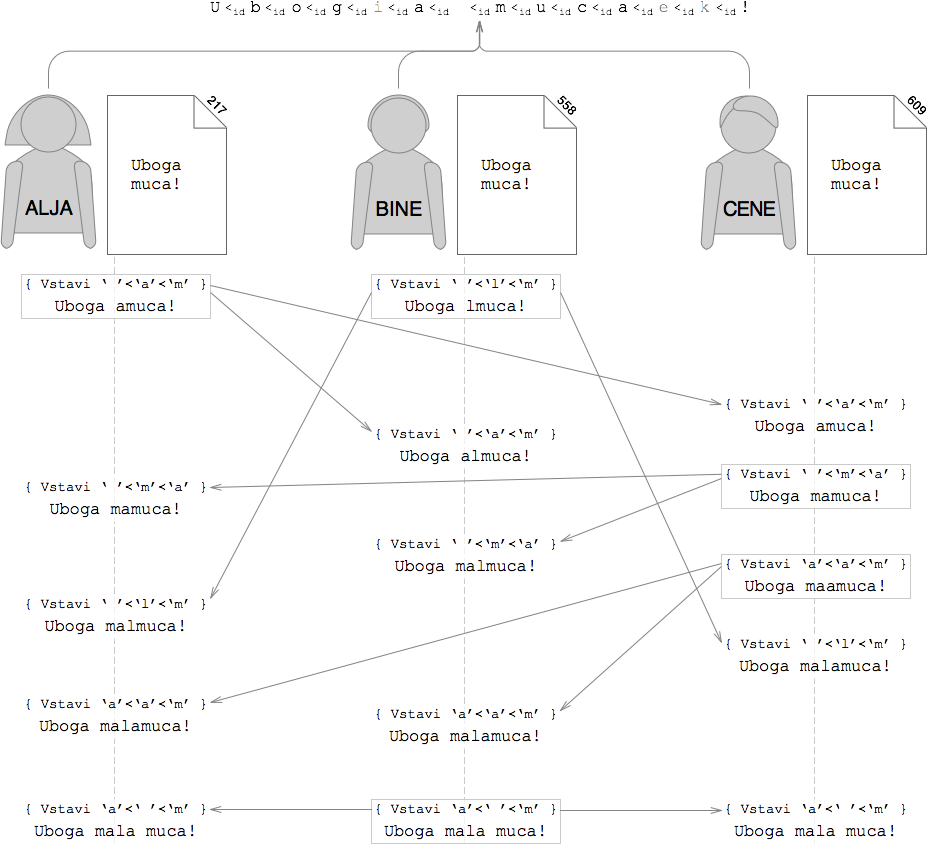
\includegraphics[width=13cm]{woot6.png}
\end{center}
\caption{Prikaz sodelovanje s protokolom WOOT preko omrežja točka-točka. Vsak od uporabnikov je vpisal svojo izbrano črko oziroma črki.}
\label{woot6}
\end{figure}

Poglejmo na Sliko \ref{woot6} kaj se je zgodilo. Alja in Bine sta hkrati vpisala črki {\tt a} in {\tt l} pred začetek besede {\tt muca}. Nato se je aktiviral Cene in dodal še njegov prispevek s črkami {\tt m} in {\tt a}. Da je stavek brez pravopisanih napak, je na koncu Bine vpisal še presledek. Ker ta zadnja sprememba ni nič posebenga, jo odmislimo pri razmišljanju. Operacije označene v pravokotnikih so se integrirala najprej lokalno, nato pa so bile poslane naprej po omrežju. Puščice prikazujejo pošljanje operacije še drugim dvema uporabnikoma. Uporabniki so skupno naredili štiri vstavljanja črka {\tt m}, {\tt a}, {\tt l} in {\tt a}. Kljub temu, da se pri nobenem uporabniku niso črke vstavljale v tem zaporedju, vsi na koncu vidijo isti pravilen rezultat.

Za študijo primera vzemimo Ceneta. Najprej je od Alje prejel, da mora med presledek in črko {\tt m} vpisati črko {\tt a}. Ker sam ni še nič urejal, je to operacijo integriral brez težav. Nato je naredil dve lokalni integraciji. Pred prej vpisani {\tt a} od Alje je vpisal črko {\tt m}, za njim pa črko {\tt a}. Ker je šlo za lokalno integracijo, jo je lahko izvedel brez težav. Cene je imel v tem trenutku v svojem dokumentu nesmiselen stavek “{\tt Uboga maamuca!}”. Nato je prejel Binetovo spremembo {\tt \{ Vstavi ‘ ’$\prec$‘l’$\prec$‘m’ \}}. Zmeden bralec bi lahko mislil, da je pravilna integracija črke {\tt l} na lokacijo 7. Nastal bi stavek “{\tt Uboga lmaamuca!}”. Res je, da Cene sprejme informacijo, da mora črko {\tt l} locirati med presledek in m, vendar je ta informacija podana z identifikaciskimi številkami in ne z alfanumeričnimi znaki kot smo to že omenil. Po tem premisleku nam je jasno, da mora biti črka {\tt l} integrirana med presledek in drugi {\tt m} v stavku. Potemtakem so kar štiri možnosti kam se lahko integrira {\tt l}. Nastanejo lahko variante:

\begin{itemize}
	\item {\tt Uboga lmaamuca!}
	\item {\tt Uboga mlaamuca!}
	\item {\tt Uboga malamuca!}
	\item {\tt Uboga maalmuca!}
\end{itemize}

Kako urejevalnik ve, kam go mora postaviti? Da bomo lažje razrešili ta problem si poglejmo Sliko \ref{woot7}.

\begin{figure}[placement h]
\begin{center}
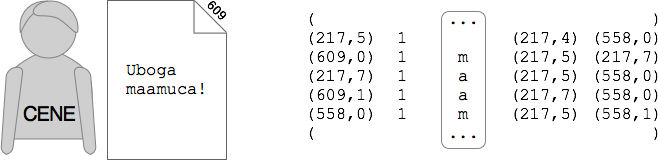
\includegraphics[width=13cm]{woot7.png}
\end{center}
\caption{Del Cenetovega dokumenta pred integracijo črke {\tt l}.}
\label{woot7}
\end{figure}

Prikazane so konfliktne črke v Cenetovem dokumentu tik pred integracijo črke {\tt l (558,7)}. Postopek je sledeč. Vzamemo seznam črk, ki so znotraj meje med katere bi se moral integrirati {\tt l}. Dobimo črke {\tt m (609,0)}, {\tt a (217,7)} in {\tt a (609,1)}. Iz tega seznama odstranimo črke, ki imajo prejšnjega ali naslednjega soseda znoraj meje med katere bi se moral integrirati {\tt l}. Ostane nam samo črka {\tt a (217,7)}. Primerjamo identifikacijsko številko črke {\tt a} in črke {\tt l}. Ker je 217 manjše od 558, se bo črka {\tt l (558,7)} postavila desno od črke {\tt a (217,7)}. Primerjavo moramo nadaljevati z vsemi črkami do meje. Naslednja po vrsti je črka {\tt a (609,1)}. Ker je 558 manjše od 609, se bo črka {\tt l (558,7)} postavila levo od črke {\tt a (609,1)}. Primerjanje zaključeno. Pravilna oblika stavka je “{\tt Uboga malamuca!}”.

Ko se integrira še Binetov presledek, dobimo “{\tt Uboga mala muca!}”.

%%%%%%%%%%%%%%%%%%%%%%%%%%%%%%%%%%%%%%%%%%%%%%%%%%%%%%%%%%%%%%%%%%%%%%%%%%%%%%%%%%%%%%%%%%%%%%%%%%%%%%%%%%%%%%%%%%
\chapter{Primerjava algoritmov}

Phasellus felis diam, molestie in laoreet ac, vestibulum at nunc.

%%%%%%%%%%%%%%%%%%%%%%%%%%%%%%%%%%%%%%%%%%%%%%%%%%%%%%%%%%%%%%%%%%%%%%%%%%%%%%%%%%%%%%%%%%%%%%%%%%%%%%%%%%%%%%%%%%
\section{Delovanje pri počasni povezavi}

Cras dictum laoreet mi at lacinia. Sed nec volutpat leo. Nulla facilisi. Sed at orci ante. Integer id dui lectus. Maecenas sagittis, libero molestie varius lobortis, urna sapien congue magna, non commodo est turpis quis lacus. Vestibulum molestie tristique auctor.

%%%%%%%%%%%%%%%%%%%%%%%%%%%%%%%%%%%%%%%%%%%%%%%%%%%%%%%%%%%%%%%%%%%%%%%%%%%%%%%%%%%%%%%%%%%%%%%%%%%%%%%%%%%%%%%%%%
\section{Iskanje razlik ali poslušalci akcij}

Donec sed eros venenatis, facilisis quam non, aliquam libero. Vivamus in vulputate leo. Integer tellus ipsum, venenatis ut sagittis eu, elementum eu nisi. Curabitur sit amet consectetur sem. Nulla in velit sed arcu ultrices fermentum. Fusce in est at sem interdum sagittis vel ac tellus.

%%%%%%%%%%%%%%%%%%%%%%%%%%%%%%%%%%%%%%%%%%%%%%%%%%%%%%%%%%%%%%%%%%%%%%%%%%%%%%%%%%%%%%%%%%%%%%%%%%%%%%%%%%%%%%%%%%
\section{Zahtevnost algoritma}

Maecenas consequat adipiscing ligula, a imperdiet ligula tincidunt ut. Sed a tristique quam. Sed quis posuere lorem. In suscipit lacus eu velit pellentesque scelerisque. Etiam pretium in mi vel placerat. Nunc at ultrices lacus, id tincidunt magna.

%%%%%%%%%%%%%%%%%%%%%%%%%%%%%%%%%%%%%%%%%%%%%%%%%%%%%%%%%%%%%%%%%%%%%%%%%%%%%%%%%%%%%%%%%%%%%%%%%%%%%%%%%%%%%%%%%%
\section{Model odjemalec-strežnik ali decentralizacija}

Proin adipiscing ac dui vel rutrum. Aenean sit amet placerat nibh. Nulla tempus tristique tortor in auctor. Fusce volutpat mattis fermentum. Maecenas accumsan nibh ut nisi consequat, eget blandit augue auctor. Aenean ac elementum mi. Aenean eu mattis ipsum. Vivamus dolor ipsum, aliquet id dapibus mattis, pretium vel enim.

%%%%%%%%%%%%%%%%%%%%%%%%%%%%%%%%%%%%%%%%%%%%%%%%%%%%%%%%%%%%%%%%%%%%%%%%%%%%%%%%%%%%%%%%%%%%%%%%%%%%%%%%%%%%%%%%%%
\section{Konsistentnost}

Mauris imperdiet ut leo a tempus. Aliquam tempor condimentum massa, at varius diam egestas nec. Mauris eu sem at odio sagittis porta. Curabitur quis rhoncus magna, vitae dignissim enim.

%%%%%%%%%%%%%%%%%%%%%%%%%%%%%%%%%%%%%%%%%%%%%%%%%%%%%%%%%%%%%%%%%%%%%%%%%%%%%%%%%%%%%%%%%%%%%%%%%%%%%%%%%%%%%%%%%%
\section{Shranjevanje podatkov}

Quisque ut velit bibendum, convallis urna vitae, tempor felis. Fusce cursus condimentum nisl, accumsan pharetra lorem iaculis sit amet. In ac lectus est. Nulla facilisi. Vivamus ornare justo id neque interdum, auctor ornare turpis cursus.

%%%%%%%%%%%%%%%%%%%%%%%%%%%%%%%%%%%%%%%%%%%%%%%%%%%%%%%%%%%%%%%%%%%%%%%%%%%%%%%%%%%%%%%%%%%%%%%%%%%%%%%%%%%%%%%%%%
\chapter{Algoritmi za iskanje razlik v besedilu}

Nulla vel lorem erat. Nullam convallis molestie mauris non vulputate. Fusce sagittis purus non mi interdum, ac tempor nunc vulputate. Vivamus tempor diam a laoreet porta. Aliquam adipiscing elit vel risus accumsan, eget lacinia felis rutrum. Mauris ornare mattis vestibulum. Proin adipiscing semper turpis, eleifend sollicitudin tortor aliquam eget.

%%%%%%%%%%%%%%%%%%%%%%%%%%%%%%%%%%%%%%%%%%%%%%%%%%%%%%%%%%%%%%%%%%%%%%%%%%%%%%%%%%%%%%%%%%%%%%%%%%%%%%%%%%%%%%%%%%
\chapter{Urejevalniki v realnem času}

Vestibulum euismod nisl orci. Curabitur consectetur, nibh vel tristique pretium, enim magna hendrerit tortor, non rutrum risus nibh et urna. Vivamus a ornare libero. Integer vitae tortor tincidunt, placerat mauris ac, molestie risus. Pellentesque ipsum neque, molestie nec malesuada blandit, fringilla cursus sapien. Sed sed risus lacinia, tempus tortor at, cursus metus. In lacinia elit vel est varius, feugiat faucibus libero vulputate. Nam molestie enim ut interdum venenatis. Donec dolor arcu, blandit et tempor nec, cursus a leo. Phasellus id sollicitudin sapien. Aenean placerat adipiscing metus eget rutrum.

%%%%%%%%%%%%%%%%%%%%%%%%%%%%%%%%%%%%%%%%%%%%%%%%%%%%%%%%%%%%%%%%%%%%%%%%%%%%%%%%%%%%%%%%%%%%%%%%%%%%%%%%%%%%%%%%%%
\chapter{Poskus implementacije OT}

Sed nec luctus elit. Etiam feugiat, ipsum at fringilla iaculis, ligula massa auctor lorem, quis viverra ligula quam ut orci. Ut faucibus consectetur velit vel adipiscing. Aliquam nec metus sapien. Morbi nec lobortis ipsum. Etiam vehicula, libero dapibus pulvinar pretium, orci nunc aliquam leo, id bibendum lacus diam id quam. Etiam at lectus ac mi malesuada ultricies. Cras id venenatis nisl. Mauris ullamcorper felis eget arcu rhoncus ullamcorper. Nullam sollicitudin justo in orci iaculis, eget tristique tellus adipiscing. Sed at bibendum felis, viverra mollis est. Proin convallis felis eget augue condimentum, at placerat sem porttitor. Sed turpis nulla, fringilla sit amet ultrices id, condimentum ut massa. Pellentesque nec augue a mauris commodo suscipit et in ante. Praesent mollis et diam nec fermentum.

\begin{lstlisting}[caption={Interdum pretium}, label={lst:codeJavaScript}, title={Exampelus \ref{lst:codeJavaScript}: Interdum pretium}]
function cache_add () {
	var self = this;

	@\label{lst:codeJavaScript_mark}@self.cache.add(self.user._id + '_testing', self.resource('sl', 'session_dafaq'));

	self.json({
			status: 'okay',
			text: self.resource('sl', 'cache_has_been_successfully_set')
	}); return;
}
\end{lstlisting}

Pellentesque egestas orci quis dui tincidunt \ref{lst:codeJavaScript} io linus \ref{lst:codeJavaScript_mark} fringilla. Vivamus ac libero arcu. Mauris hendrerit massa eros. Morbi augue ligula, viverra sed volutpat at, pharetra ut erat. Integer consectetur tristique diam, vulputate placerat urna fermentum eu. Ut feugiat ligula a quam venenatis gravida. Ut elementum fermentum sapien, at posuere purus lacinia non. Mauris ante nunc, sodales eu pretium vitae, ultrices ac turpis.

%%%%%%%%%%%%%%%%%%%%%%%%%%%%%%%%%%%%%%%%%%%%%%%%%%%%%%%%%%%%%%%%%%%%%%%%%%%%%%%%%%%%%%%%%%%%%%%% sklpne ugotovitve
\chapter{Sklepne ugotovitve}

Nam semper augue at rhoncus laoreet. Nunc non aliquet risus. Curabitur dictum, nisl nec interdum pretium, dui quam vehicula urna, vel porta nunc est rutrum tellus. Aliquam condimentum pharetra sem, sed sodales massa viverra id. Nam aliquam faucibus egestas. Cras viverra non augue sed sagittis. Nam et elit a tortor aliquet laoreet. Pellentesque congue, risus ultricies rhoncus tincidunt, quam libero tempor tellus, sit amet bibendum velit augue eleifend lectus. Integer lorem nulla, placerat varius faucibus eu, cursus tempor purus. Cras at suscipit elit. Nam varius in ipsum eget tristique. Nulla ac nulla rutrum, vulputate lacus ac, dignissim ligula.

%%%%%%%%%%%%%%%%%%%%%%%%%%%%%%%%%%%%%%%%%%%%%%%%%%%%%%%%%%%%%%%%%%%%%%%%%%%%%%%%%%%%%%%%%%%%%%%%%%%%%%% literatura
\addcontentsline{toc}{chapter}{Literatura}
\begin{thebibliography}{99}

\bibitem{ccigs} C.A. Ellis, S.J. Gibbs. “Concurrency Control in Groupware Systems”.
\\\url{http://www-ihm.lri.fr/~mbl/ENS/CSCW/2012/papers/Ellis-SIGMOD89.pdf}

\bibitem{hllbw} D. A. Nichols, P. Curtis, M. Dixon, J. Lamping. “High-Latency, Low-Bandwidth Windowing in the Jupiter Collaboration System”.
\\\url{http://lively-kernel.org/repository/webwerkstatt/!svn/bc/15693/projects/Collaboration/paper/Jupiter.pdf}

\bibitem{sigce} The Special Interest Group on Collaborative Computing
\\\url{http://cooffice.ntu.edu.sg/sigce/}

\bibitem{wave} D. Wang, A. Mah, S. Lassen. Google Wave Operational Transformation.
\\\url{http://www.waveprotocol.org/whitepapers/operational-transform}

\bibitem{share} J. Gentle. ShareJS - Live concurrent editing in your app.
\\\url{http://sharejs.org/}

\bibitem{node} Joyent, Inc., R. Dahl. Node.js.
\\\url{http://nodejs.org/}

\bibitem{problem} The Dojo Fundation. Open Cooperative Web Framework.
\\\url{http://opencoweb.org/ocwdocs/intro/openg.html}

\bibitem{diffsync} Neil Fraser. Differential Synchronization.
\\\url{https://neil.fraser.name/writing/sync/}

\bibitem{gdocs22} J. Day-Richter. What’s different about the new Google Docs: Conflict resolution.
\\\url{http://googledocs.blogspot.com/2010/09/whats-different-about-new-google-docs_22.html}

\bibitem{gdocs23} J. Day-Richter. What’s different about the new Google Docs: Making collaboration fast.
\\\url{http://googledocs.blogspot.com/2010/09/whats-different-about-new-google-docs_23.html}

\bibitem{woot} G. Oster, P. Urso, P. Molli, A. Imine. Real time group editors without Operational transformation.
\\\url{http://hal.inria.fr/docs/00/07/12/40/PDF/RR-5580.pdf}

\end{thebibliography}

%%%%%%%%%%%%%%%%%%%%%%%%%%%%%%%%%%%%%%%%%%%%%%%%%%%%%%%%%%%%%%%%%%%%%%%%%%%%%%%%%%%%%%%%%%%%%%%%%%%%%%%%%%%%%%%%%%
\end{document}